\documentclass[11pt]{book}

\setlength{\textheight}{8.5in}
\setlength{\oddsidemargin}{-0.2in}
\setlength{\evensidemargin}{0in}
\setlength{\textwidth}{6.75in}
\setlength{\topmargin}{0.1in}

\usepackage{color}
\usepackage{amssymb,amsthm,amsmath,amsfonts,latexsym}
\usepackage{graphics}
\usepackage{graphicx}
\usepackage{setspace}
\usepackage[square,numbers,sort&compress]{natbib}
\usepackage{verbatim}
\usepackage{mathrsfs}

\allowdisplaybreaks[1]

\begin{document}

\tableofcontents
\newpage

%%%%%%%%%%%%%%%%%%%%%%%%%%%%%%%%%%%%%%%%%%%%%%%%%%%%%%%%%%%%%%%%%%%%%%%%%%%%%%%%%%%%%%%%%%%%%%%%%%
%%%%%%%%%%%%%%%%%%%%%%%%%%%%%%%%%%%%%%%%%%%%%%%%%%%%%%%%%%%%%%%%%%%%%%%%%%%%%%%%%%%%%%%%%%%%%%%%%%
%%%%%%%%%%%%%%%%%%%%%%%%%%%%%%%%%%%%%%%%%%%%%%%%%%%%%%%%%%%%%%%%%%%%%%%%%%%%%%%%%%%%%%%%%%%%%%%%%%
%%%%%%%%%%%%%%%%%%%%%%%%%%%%%%%%%%%%%%%%%%%%%%%%%%%%%%%%%%%%%%%%%%%%%%%%%%%%%%%%%%%%%%%%%%%%%%%%%%

\chapter{Force Field}

%%%%%%%%%%%%%%%%%%%%%%%%%%%%%%%%%%%%%%%%%%%%%%%%%%%%%%%%%%%%%%%%%%%%%%%%%%%%%%%%%%%%%%%%%%%%%%%%%%
%%%%%%%%%%%%%%%%%%%%%%%%%%%%%%%%%%%%%%%%%%%%%%%%%%%%%%%%%%%%%%%%%%%%%%%%%%%%%%%%%%%%%%%%%%%%%%%%%%
%%%%%%%%%%%%%%%%%%%%%%%%%%%%%%%%%%%%%%%%%%%%%%%%%%%%%%%%%%%%%%%%%%%%%%%%%%%%%%%%%%%%%%%%%%%%%%%%%%

\section{Background}

The relationship between coordinates of atoms in a system and its energy is an essential part of any computational study based on atomic models. The potential energy function (force field) \cite{MacKerellJPC98,MacKerellJCC04} is used to calculate the potential energy of the system and to evaluate all the forces acting on all the atoms in the system. The force-field is the potential energy (i.e. function of coordinates) specified in terms of some constant parameters (parameters of the force field). A full-atomic potential energy function $V$ is usually given by the sum of the bonded terms ($V_{b}$) and non-bonded terms ($V_{nb}$) \cite{Charmm83,Charmm09,Namd05,Gromacs08,Amber05}, i.e.
%%
\begin{equation}\label{eq:ff}
V = V_{b} + V_{nb},
\end{equation}
%%
where the bonded potential includes harmonic (covalent) bond part, harmonic angle and two types of torsion (dihedral) angles (proper and improper angles):
%%
\begin{equation}\label{eq:ff-bonded}
V_{b} = \sum_{bonds}\frac{k_b}{2}(b-b_0)^2 + \sum_{angles}\frac{k_{\theta}}{2}(\theta-\theta_0)^2 + \sum_{dihedrals}k_{\phi}(1-cos(n\phi - \phi_0)) + \sum_{impropers}\frac{k_{\psi}}{2}(\psi-\psi_0)^2
\end{equation}
%%
For example, $b$ and $\theta$ represent distance between two atoms and angle between two adjacent bonds; $\phi$ and $\psi$ are dihedral (torsion) angles. These can be evaluated for all the atoms from their current positions. Also, $k_b$, $k_{\theta}$, $k_{\phi}$, and $k_{\psi}$ are the spring constants, associated with bond vibrations, bending of bond angles, and conformational fluctuations in dihedral and improper angles around some equilibrium values $b_0$, $\theta_0$, $\phi_0$, and $\psi_0$, respectively. Importantly, each force-field has its own set of these parameters, which vary for different types of atoms \cite{Charmm83,GromacsManual}. Some force-fields might also include Urey-Bradley angle corrections \cite{Charmm83} and/or dihedral CMAP correction terms \cite{MacKerellJACS04,MacKerellJCC04-CMAP,Charmm09}. The non-bonded part of the potential energy function is represented by the electrostatic and Van-der-Waals potentials, i.e.
%%
\begin{equation}\label{eq:ff-nb}
V_{nb} = \sum_{i,j}\left(\frac{q_{i}q_{j}}{4\pi\varepsilon_{0}\varepsilon r_{ij}} + \varepsilon_{ij}\left[\left(\frac{R^{min}_{ij}}{r_{ij}}\right)^{12}-2\left(\frac{R^{min}_{ij}}{r_{ij}}\right)^{6}\right]\right)
\end{equation}
%%
where $r_{ij}$ is a distance between two interacting atoms, $q_{i}$ and $q_{j}$ are their charges; $\varepsilon$ and $\varepsilon_{0}$ are electric and dielectric constant; $\varepsilon_{ij}=\sqrt{\varepsilon_i\varepsilon_j}$ and $R_{ij}^{min} = (R_{i}^{min} + R_{j}^{min})/2$ are Van-der-Waals parameters for atoms $i$ and $j$. Early potential energy functions also included explicitly the hydrogen bonds potentials \cite{Charmm83}, which later have been dropped due to improved parametrization of electrostatics \cite{Charmm09}.

%%%%%%%%%%%%%%%%%%%%%%%%%%%%%%%%%%%%%%%%%%%%%%%%%%%%%%%%%%%%%%%%%%%%%%%%%%%%%%%%%%%%%%%%%%%%%%%%%%
%%%%%%%%%%%%%%%%%%%%%%%%%%%%%%%%%%%%%%%%%%%%%%%%%%%%%%%%%%%%%%%%%%%%%%%%%%%%%%%%%%%%%%%%%%%%%%%%%%
%%%%%%%%%%%%%%%%%%%%%%%%%%%%%%%%%%%%%%%%%%%%%%%%%%%%%%%%%%%%%%%%%%%%%%%%%%%%%%%%%%%%%%%%%%%%%%%%%%

\section{Covalent bonds}
Covalent bonds are usually described by a harmonic potential:
%%
\begin{equation}\label{eq:ff-covalent}
V_{bonds} = \sum_{bonds}k_b(b-b_0)^2
\end{equation}
%%
%%
\begin{equation}\label{eq:ff-gradr}
\nabla_{l}r_{ij} =
\begin{cases}
	\frac{\vec{r}_{ij}}{r_{ij}} & \text{when } i = l\\
	\frac{\vec{r}_{ji}}{r_{ij}} & \text{when } j = l\\
	0                           & \text{when } i \ne l \text{ and } j \ne l
\end{cases}
\end{equation}
%%

%%%%%%%%%%%%%%%%%%%%%%%%%%%%%%%%%%%%%%%%%%%%%%%%%%%%%%%%%%%%%%%%%%%%%%%%%%%%%%%%%%%%%%%%%%%%%%%%%%
%%%%%%%%%%%%%%%%%%%%%%%%%%%%%%%%%%%%%%%%%%%%%%%%%%%%%%%%%%%%%%%%%%%%%%%%%%%%%%%%%%%%%%%%%%%%%%%%%%
%%%%%%%%%%%%%%%%%%%%%%%%%%%%%%%%%%%%%%%%%%%%%%%%%%%%%%%%%%%%%%%%%%%%%%%%%%%%%%%%%%%%%%%%%%%%%%%%%%

\section{Angle potential}
%%
\begin{figure}[h]
\begin{center}
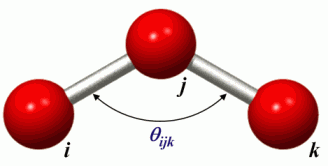
\includegraphics[width=2in]{Figures/PotScheme/pot-angle.png}
\end{center}
\caption{A schematic representation of a three atoms, interacting through angle potential. A triplet of atoms $(i,j,k)$ and the current angle $\theta_{ijk}$ are shown.}
\label{fig:pot-angle}
\end{figure}
%%
As it is shown in Eq.~\ref{eq:ff-nb}, angle potential is described by following relalation:
%%
\begin{equation}\label{eq:ff-angles1}
V_{angles} = \sum_{angles}\frac{k_{\theta}}{2}(\theta-\theta_0)^2
\end{equation}
%%
Introducing a triplet $(i,j,k)$ of atoms, involved in a particular angle (Fig.~\ref{fig:pot-angle}) and a set of angles in a system, $A$, one can re-write the equation above as:
%%
\begin{equation}\label{eq:ff-angles2}
V_{angles} = \sum_{(i,j,k) \in A}\frac{k_{ijk}^{\theta}}{2}(\theta_{ijk}-\theta^0_{ijk})^2
\end{equation}
%%
The force, acting on a particular atom $l$ due to the angle potential is then:
%%
\begin{equation}\label{eq:ff-angles3}
\vec{f}_{l}=-\nabla_{l}V_{angles} = -\nabla_{l}\left(\sum_{(i,j,k) \in A}\frac{k_{ijk}^{\theta}}{2}(\theta_{ijk}-\theta^0_{ijk})^2\right) = -\sum_{(i,j,k) \in A}k_{ijk}^{\theta}(\theta_{ijk}-\theta^0_{ijk})\nabla_{l}\theta_{ijk}
\end{equation}
%%
Since numericaly it is easier to compute $\cos\theta_{ijk}$ and $\sin\theta_{ijk}$, let us switch to a $\cos$ and $\sin$ representation as follows:
%%
\begin{equation}\label{eq:ff-angles4}
\theta_{ijk}=\arccos\left(\cos\theta_{ijk}\right),
\end{equation}
%%
and
%%
\begin{equation}\label{eq:ff-angles5}
\nabla_{l}\theta_{ijk} = \nabla_{l}\left(\arccos\left(\cos\theta_{ijk}\right)\right) = -\frac{1}{\sqrt{1-\cos^{2}\theta_{ijk}}}\nabla_{l}\cos\theta_{ijk} = -\frac{\nabla_{l}\cos\theta_{ijk}}{\sin\theta_{ijk}}.
\end{equation}
%%
Let us denote vectors that connect particles $i$, $j$ and $k$ in a triplet as $\vec{r}_{ji}=\vec{r}_{i}-\vec{r}_{j}$ and $\vec{r}_{jk}=\vec{r}_{k}-\vec{r}_{j}$. Then:
%%
\begin{equation}\label{eq:ff-angles6}
\cos\theta_{ijk}=\frac{\vec{r}_{ji}\cdot\vec{r}_{jk}}{|\vec{r}_{ji}||\vec{r}_{jk}|}=\frac{\vec{r}_{ji}\cdot\vec{r}_{jk}}{r_{ji}r_{jk}}
\end{equation}
%%
Here, $\vec{r}_{ji}\cdot\vec{r}_{jk}$ is a dot product of vectors $\vec{r}_{ji}$ and $\vec{r}_{jk}$. It is clear, that $\nabla_{l}\cos\theta_{ijk}$ will vanish if $l$ does not belong to the triplet $(i,j,k)$. Considering all three cases ($l=i$, $l=j$ and $j=k$) separately and using Eq.~\ref{eq:ff-angles6} one gets:
\begin{equation}\label{eq:ff-angles7}
\begin{split}
\nabla_{l}\cos\theta_{ijk}\bigg|_{l=i}&=\nabla_{l}\left(\frac{\vec{r}_{ji}\cdot\vec{r}_{jk}}{r_{ji}r_{jk}}\right)\bigg|_{l=i}=\left(\frac{1}{r_{ji}r_{jk}}\nabla_{l}\left(\vec{r}_{ji}\cdot\vec{r}_{jk}\right)-\frac{\vec{r}_{ji}\cdot\vec{r}_{jk}}{r_{ji}^{2}r_{jk}}\nabla_{l}r_{ji}\right)\bigg|_{l=i}=\\
&=\frac{1}{r_{ji}r_{jk}}\vec{r}_{jk}-\frac{\vec{r}_{ji}\cdot\vec{r}_{jk}}{r_{ji}^{2}r_{jk}}\frac{\vec{r}_{ji}}{r_{ji}}=\frac{1}{r_{ji}}\left[\frac{\vec{r}_{jk}}{r_{jk}}-\cos\theta_{ijk}\frac{\vec{r}_{ji}}{r_{ji}}\right]\text{,}\\
\nabla_{l}\cos\theta_{ijk}\bigg|_{l=k}&=\nabla_{l}\left(\frac{\vec{r}_{ji}\cdot\vec{r}_{jk}}{r_{ji}r_{jk}}\right)\bigg|_{l=k}=\left(\frac{1}{r_{ji}r_{jk}}\nabla_{l}\left(\vec{r}_{ji}\cdot\vec{r}_{jk}\right)-\frac{\vec{r}_{ji}\cdot\vec{r}_{jk}}{r_{ji}r_{jk}^{2}}\nabla_{l}r_{jk}\right)\bigg|_{l=k}=\\
&=\frac{1}{r_{ji}r_{jk}}\vec{r}_{ji}-\frac{\vec{r}_{ji}\cdot\vec{r}_{jk}}{r_{ji}r_{jk}^{2}}\frac{\vec{r}_{jk}}{r_{jk}}=\frac{1}{r_{jk}}\left[\frac{\vec{r}_{ji}}{r_{ji}}-\cos\theta_{ijk}\frac{\vec{r}_{jk}}{r_{jk}}\right]\text{, and}\\
\nabla_{l}\cos\theta_{ijk}\bigg|_{l=j}&=\nabla_{l}\left(\frac{\vec{r}_{ji}\cdot\vec{r}_{jk}}{r_{ji}r_{jk}}\right)\bigg|_{l=j}=\left(\frac{1}{r_{ji}r_{jk}}\nabla_{l}\left(\vec{r}_{ji}\cdot\vec{r}_{jk}\right)-\frac{\vec{r}_{ji}\cdot\vec{r}_{jk}}{r_{ji}^{2}r_{jk}}\nabla_{l}r_{ji}-\frac{\vec{r}_{ji}\cdot\vec{r}_{jk}}{r_{ji}r_{jk}^{2}}\nabla_{l}r_{jk}\right)\bigg|_{l=j}=\\
&=-\frac{1}{r_{ji}r_{jk}}\vec{r}_{jk}-\frac{1}{r_{ji}r_{jk}}\vec{r}_{ji}+\frac{\vec{r}_{ji}\cdot\vec{r}_{jk}}{r_{ji}^{2}r_{jk}}\frac{\vec{r}_{ji}}{r_{ji}}+\frac{\vec{r}_{ji}\cdot\vec{r}_{jk}}{r_{ji}r_{jk}^{2}}\frac{\vec{r}_{jk}}{r_{jk}}=\\
&=\frac{1}{r_{ji}}\left[\cos\theta_{ijk}\frac{\vec{r}_{ji}}{r_{ji}}-\frac{\vec{r}_{jk}}{r_{jk}}\right] + \frac{1}{r_{jk}}\left[\cos\theta_{ijk}\frac{\vec{r}_{jk}}{r_{jk}}-\frac{\vec{r}_{ji}}{r_{ji}}\right]=\\
&=-\nabla_{l}\cos\theta_{ijk}\bigg|_{l=i}-\nabla_{l}\cos\theta_{ijk}\bigg|_{l=k}
\end{split}
\end{equation}
%%
Summirizing Eqs.~\ref{eq:ff-angles3}, \ref{eq:ff-angles5} and \ref{eq:ff-angles7}, one can compute three components of force $\vec{f}_{i}$, $\vec{f}_{j}$ and $\vec{f}_{k}$, acting on each atom in the angle triplet $(i,j,k)$ due to the angle potential between atoms $i$, $j$ and $k$ using the following relations:
\begin{equation}\label{eq:ff-angles8}
\begin{split}
\vec{f}_{i}&=k_{ijk}^{\theta}(\theta_{ijk}-\theta^0_{ijk})\left(-\frac{1}{\sin\theta_{ijk}}\right)\frac{1}{r_{ji}}\left[\cos\theta_{ijk}\frac{\vec{r}_{ji}}{r_{ji}}-\frac{\vec{r}_{jk}}{r_{jk}}\right]\\
\vec{f}_{k}&=k_{ijk}^{\theta}(\theta_{ijk}-\theta^0_{ijk})\left(-\frac{1}{\sin\theta_{ijk}}\right)\frac{1}{r_{jk}}\left[\cos\theta_{ijk}\frac{\vec{r}_{jk}}{r_{jk}}-\frac{\vec{r}_{ji}}{r_{ji}}\right]\\
\vec{f}_{j}&=-\vec{f}_{i}-\vec{f}_{k}
\end{split}
\end{equation}

%%%%%%%%%%%%%%%%%%%%%%%%%%%%%%%%%%%%%%%%%%%%%%%%%%%%%%%%%%%%%%%%%%%%%%%%%%%%%%%%%%%%%%%%%%%%%%%%%%
%%%%%%%%%%%%%%%%%%%%%%%%%%%%%%%%%%%%%%%%%%%%%%%%%%%%%%%%%%%%%%%%%%%%%%%%%%%%%%%%%%%%%%%%%%%%%%%%%%
%%%%%%%%%%%%%%%%%%%%%%%%%%%%%%%%%%%%%%%%%%%%%%%%%%%%%%%%%%%%%%%%%%%%%%%%%%%%%%%%%%%%%%%%%%%%%%%%%%

\section{Van-der-Waals interactions}

The formal definition of the Lennard-Jones potential that describes Van-der-Waals interactions reads:
\begin{equation}\label{eq:pot-lj}
V_{LJ}=\sum_{ij}V_{LJ}^{ij}=\sum_{ij}\varepsilon_{ij}\left[\left(\frac{\sigma_{ij}}{r_{ij}}\right)^{12}-2\left(\frac{\sigma_{ij}}{r_{ij}}\right)^{6}\right].
\end{equation}
Then, the force acting on the particle due to this potential is:
\begin{equation}\label{eq:f-lj}
\vec{f}^{LJ}_{ij}=-\nabla_{i}V_{LJ}^{ij}=\varepsilon_{ij}\left[12\frac{\sigma_{ij}^{12}}{r_{ij}^{13}}-12\frac{\sigma_{ij}^{6}}{r_{ij}^{7}}\right]\frac{\vec{r}_{ij}}{r_{ij}}=12\varepsilon_{ij}\left(\frac{\sigma_{ij}}{r_{ij}}\right)^{6}\left[\left(\frac{\sigma_{ij}}{r_{ij}}\right)^{6}-1\right]\frac{\vec{r}_{ij}}{r_{ij}^{2}}.
\end{equation}
Evaluation of the $\vec{f}^{LJ}_{ij}$ requires $N^{2}$ binary forces to be computed. If a big atomistic system is considered, this can be a prohibitive factor for a long-timescale simulations. Most common work-around of this problem is to use the fact that the potential vanishes rapidly with distance. This allows one to cut the potential function off at some distance and, instead of computing potential for all $N^{2}$ binary pairs, consider only those particles that are close to the particle in question. This requires two more features to be implemented. First, a neighbours list - a list of particles that are close to the particle in question has to be constructed. Second, since the potential is not zero at any given distance, but rather assimptotically goes to zero, some changes have to be done to the potential function so that the value of the potential energy and its derivative is zero at the introduced cut-off distance. Later can be done using shifted or switched potential.

%%%%%%%%%%%%%%%%%%%%%%%%%%%%%%%%%%%%%%%%%%%%%%%%%%%%%%%%%%%%%%%%%%%%%%%%%%%%%%%%%%%%%%%%%%%%%%%%%%
%%%%%%%%%%%%%%%%%%%%%%%%%%%%%%%%%%%%%%%%%%%%%%%%%%%%%%%%%%%%%%%%%%%%%%%%%%%%%%%%%%%%%%%%%%%%%%%%%%
%%%%%%%%%%%%%%%%%%%%%%%%%%%%%%%%%%%%%%%%%%%%%%%%%%%%%%%%%%%%%%%%%%%%%%%%%%%%%%%%%%%%%%%%%%%%%%%%%%

\section{Switching function}

Consider an arbitraty binary potential $V({\bf r})$ (${\bf r}=(\vec{r}_{1},\vec{r}_{2},\ldots,\vec{r}_{N}$)) that undergo a swithing function $sw({\bf r})$:
%%
\begin{equation}\label{eq:sw1}
V^{sw}({\bf r})=V({\bf r})sw({\bf r})=\sum_{i=1}^{N}\sum_{j=1}^{N}V_{ij}(r_{ij})sw_{ij}(r_{ij})
\end{equation}
%%
According to the product rule, the atomic force acting on $l$-th particle due to this potential will then be:
%%
\begin{equation}\label{eq:sw2}
\begin{split}
\vec{f}_{l}({\bf r})&=-\nabla_{l} V^{sw}=-\nabla_{l}\left(\sum_{i=01}^{N}\sum_{j=1}^{N}V_{ij}(r_{ij})sw_{ij}(r_{ij})\right)=\\
&=-\sum_{i=1}^{N}\sum_{j=1}^{N}\left(\nabla_{l}V_{ij}(r_{ij})\right)sw_{ij}(r_{ij})+V_{ij}(r_{ij})\left(\nabla_{l}sw_{ij}(r_{ij})\right)
\end{split}
\end{equation}
%%
Computation of the atomic force due to the switched potential then can be done either explicetly or implicetly. In explicit approach, equation~\ref{eq:sw2} should be expanded using the actual form of the $V(r)$. In implicit approach, all four terms of a product rule formula (Eq.~\ref{eq:sw2}) should be computed independently and then used to evaluate atomic force $\vec{f}_{l}$. The choice of the approach should be made considering computational performance, depending on the mathematical form of the potential $V(r)$.

The actual form of the switching function $sw(r)$ is given by \cite{Charmm83}:
%%
\begin{equation}\label{eq:sw}
sw_{ij}(r_{ij})=
\begin{cases}
	1 & \text{when } r_{ij}\leq r_{on}\\
	\frac{\left(r_{off}^{2}-r_{ij}^{2}\right)^{2}\left(r_{off}^{2}+2r_{ij}^{2}-3r_{on}^{2}\right)}{\left(r_{off}^{2}-r_{on}^{2}\right)^{3}} & \text{when } r_{on}<r_{ij}\leq r_{off}\\
	0 & \text{when } r_{ij}>r_{off}\\
\end{cases}
\end{equation}
%%
where $r_{on}$ and $r_{off}$ are switching and cut-off distances respectively.

Since cases when $r_{ij}\leq r_{on}$ and when $r_{ij}>r_{off}$ are trivial, let us consider conditions when $r_{on}<r_{ij}\leq r_{off}$.

%%%%%%%%%%%%%%%%%%%%%%%%%%%%%%%%%%%%%%%%%%%%%%%%%%%%%%%%%%%%%%%%%%%%%%%%%%%%%%%%%%%%%%%%%%%%%%%%%%
%%%%%%%%%%%%%%%%%%%%%%%%%%%%%%%%%%%%%%%%%%%%%%%%%%%%%%%%%%%%%%%%%%%%%%%%%%%%%%%%%%%%%%%%%%%%%%%%%%

\subsection{Implicit evaluation of the switching function}

According to the product rule, one need to evaluate $V_{ij}(r_{ij})$, $\nabla_{l}V_{ij}(r_{ij})$, $sw_{ij}(r_{ij})$ and $\nabla_{l}sw_{ij}(r_{ij})$. Since all four quantities can be computed independently, here we will only consider evaluation of $sw_{ij}(r_{ij})$ and $\nabla_{l}sw_{ij}(r_{ij})$. Rearranging Eq.~\ref{eq:sw} ($r_{on}<r_{ij}\leq r_{off}$), we get:
%%
\begin{equation}\label{eq:sw3}
sw_{ij}(r_{ij})= \frac{2}{{\left(r_{off}^{2}-r_{on}^{2}\right)^{3}}}\left(r_{off}^{2}-r_{ij}^{2}\right)^{2}\left(\frac{r_{off}^{2}-3r_{on}^{2}}{2}+r_{ij}^{2}\right)
\end{equation}
%%
Since $r_{on}$ and $r_{off}$ are constant, one can use pre-computed values for:
%%
\begin{equation}\label{eq:sw4}
C^{sw}_{1} = \frac{2}{\left(r_{off}^{2}-r_{on}^{2}\right)^{3}} \text{,  }
C^{sw}_{2} = r_{off}^{2} \text{, and  }
C^{sw}_{3} = \frac{r_{off}^{2}-3r_{on}^{2}}{2}
\end{equation}
%%
Then, Eq.~\ref{eq:sw} when $r_{on}<r_{ij}\leq r_{off}$ becomes:
%%
\begin{equation}\label{eq:sw5}
sw_{ij}(r_{ij})=C^{sw}_{1}\left(C^{sw}_{2}-r_{ij}^{2}\right)^{2}\left(C^{sw}_{3}+r_{ij}^{2}\right)
\end{equation}
%%
Using Eq.~\ref{eq:sw} ($r_{on}<r_{ij}\leq r_{off}$), we also can compute $\nabla_{l}sw_{ij}(r_{ij})$:
%%
\begin{equation}\label{eq:dsw1}
\begin{split}
&\nabla_{l}sw_{ij}(r_{ij}) = \frac{1}{\left(r_{off}^{2}-r_{on}^{2}\right)^{3}}\left[2\left(r_{off}^{2}-r_{ij}^{2}\right)\left(-2r_{ij}\right)\left(r_{off}^{2}+2r_{ij}^{2}-3r_{on}^{2}\right)+\left(r_{off}^{2}-r_{ij}^2\right)^{2}4r_{ij}\right]\frac{\vec{r}_{ij}}{r_{ij}} = \\
&= \frac{1}{\left(r_{off}^{2}-r_{on}^{2}\right)^{3}}\left[-4r_{off}^{4}-8r_{off}^{2}r_{ij}^{2}+12r_{off}^{2}r_{on}^{2}+4r_{ij}^{2}r_{off}^{2}+8r_{ij}^{4}-12r_{ij}^{2}r_{on}^{2}+4r_{off}^{4}-8r_{off}^{2}r_{ij}^{2}+4r_{ij}^{4}\right]\vec{r}_{ij} = \\
&= \frac{1}{\left(r_{off}^{2}-r_{on}^{2}\right)^{3}}\left[12r_{ij}^{4}-12r_{ij}^{2}r_{off}^{2}-12r_{ij}^{2}r_{on}^{2}+12r_{off}^{2}r_{on}^{2}\right]\vec{r}_{ij} = \\
&= \frac{12}{\left(r_{off}^{2}-r_{on}^{2}\right)^{3}}\left(r_{ij}^{2}-r_{off}^{2}\right)\left(r_{ij}^2-r_{on}^{2}\right)\vec{r}_{ij}\\
\end{split}
\end{equation}
%%
Using pre-computed values for:
\begin{equation}\label{eq:dsw2}
C^{dsw} = \frac{12}{\left(r_{off}^{2}-r_{on}^{2}\right)^{3}}\text{,  } r_{off}^{2} \text{, and  } r_{on}^{2}
\end{equation}
%%
Equation~\ref{eq:dsw1} becomes:
\begin{equation}\label{eq:dsw3}
\nabla_{l}sw_{ij}(r_{ij})=C^{dsw}\left(r_{ij}^{2}-r_{off}^{2}\right)\left(r_{ij}^2-r_{on}^{2}\right)\vec{r}_{ij}
\end{equation}

%%%%%%%%%%%%%%%%%%%%%%%%%%%%%%%%%%%%%%%%%%%%%%%%%%%%%%%%%%%%%%%%%%%%%%%%%%%%%%%%%%%%%%%%%%%%%%%%%%
%%%%%%%%%%%%%%%%%%%%%%%%%%%%%%%%%%%%%%%%%%%%%%%%%%%%%%%%%%%%%%%%%%%%%%%%%%%%%%%%%%%%%%%%%%%%%%%%%%

\subsection{Explicit evaluation of the switching function}
Let us expand Eq.~\ref{eq:sw1} for the Lennard-Jones potential.


%%%%%%%%%%%%%%%%%%%%%%%%%%%%%%%%%%%%%%%%%%%%%%%%%%%%%%%%%%%%%%%%%%%%%%%%%%%%%%%%%%%%%%%%%%%%%%%%%%
%%%%%%%%%%%%%%%%%%%%%%%%%%%%%%%%%%%%%%%%%%%%%%%%%%%%%%%%%%%%%%%%%%%%%%%%%%%%%%%%%%%%%%%%%%%%%%%%%%
%%%%%%%%%%%%%%%%%%%%%%%%%%%%%%%%%%%%%%%%%%%%%%%%%%%%%%%%%%%%%%%%%%%%%%%%%%%%%%%%%%%%%%%%%%%%%%%%%%

\section{Implicit solvent models}

Accurate representation of the solvent environment is important for realistic biomolecular modeling. The most straightforward approach is to expose the biomolecule to explicetly defined water molecules. However, to avoid boundary effects, the amount of water molecules added to the system is very large. Typically, in all-atom MD simulations in explicit weater, 90\% of all the degrees of freedom correspond to the water environment. This results in the increased system size and the computational complexity, significantly slowing down the computational procedures, thus, reducing reachable timescales of simulations. This might prohibit the exploration of the biologically relevant transitions in biomolecules. Alternatively, interactions of protein and water molecules can be described by mechanical ``kicks'' of the protein atoms and Coulomb interactions that include electrostatic ``screening'' effect and entropy-driven hydrophobic effect. This approach, called implicit solvent representation \cite{ChenCOSB08,Charmm09}, involves introducing Langevin equations of motion, where random forces represent stochastic water kicks experienced by the protein molecule, and additional potential energy function to model electrostatic solvation effects. Implicit solvation models have several advantages over explicit water representations including lower computational cost, better thermodynamic sampling and more straightforward methodology for the free energy estimations.

In most implicit solvent models, the total potential energy of the solvated molecule is given by
%%
\begin{equation}\label{eq:implicit}
V_{tot} = V_{vac} + \Delta G_{solv}
\end{equation}
%%
where $V_{vac}$ is the potential energy of the molecule in vacuum (i.e. in the absence of water environment) and $\Delta G_{solv}$ is defined as the free energy of transferring the molecule from vacuum to the solvent (solvation free energy). Typically, $V_{vac}$ is computed using the molecular force field (Eqs.~\ref{eq:ff}-\ref{eq:ff-nb}), whereas $\Delta G_{solv}$ depends on the particular implicit solvent model used. $\Delta G_{solv}$ can be decomposed into the polar and non-polar parts, which represent the hydrophobic effect and electrostatic effect of the solvent, respectively. There are several different approaches for implicit water representation \cite{ChenCOSB08,Charmm09} including Solvent Accessible Surface Area (SASA) model \cite{FerraraProteins02,FraternaliJMB96} and Generilized Born (GB) model, which is based on the Generilized Born approximation of the Poisson-Boltzman equation \cite{StillJACS90,DominyJPC99,LeeJCP02,LeeJCC03,HawkinsJPC96,OnufrievJPC00}. Some other methods \cite{LazaridisProteins99} combine different descriptions of implicit solvation into hybrid models \cite{QiuJPC97}. 

%%%%%%%%%%%%%%%%%%%%%%%%%%%%%%%%%%%%%%%%%%%%%%%%%%%%%%%%%%%%%%%%%%%%%%%%%%%%%%%%%%%%%%%%%%%%%%%%%%
%%%%%%%%%%%%%%%%%%%%%%%%%%%%%%%%%%%%%%%%%%%%%%%%%%%%%%%%%%%%%%%%%%%%%%%%%%%%%%%%%%%%%%%%%%%%%%%%%%
%%%%%%%%%%%%%%%%%%%%%%%%%%%%%%%%%%%%%%%%%%%%%%%%%%%%%%%%%%%%%%%%%%%%%%%%%%%%%%%%%%%%%%%%%%%%%%%%%%

\section{SASA solvation model}

In Solvent Accessible Surface Area solvation energy approximation, it is assumed that the mean solvation energy $\Delta G_{solv}({\bf r})$ (${\bf r}=(\vec{r}_{1},\vec{r}_{2},\ldots,\vec{r}_{N}$)) is linearly related to the solvent accessible surfase area of a solute \cite{EisenbergNature86,FraternaliJMB96,FerraraProteins02}:
%%
\begin{equation}\label{eq:sasa-V}
\Delta G_{solv}^{SASA}({\bf r})=\sum_{i=1}^{N}\sigma_{i}A_{i}({\bf r}),
\end{equation}
%%
where $\sigma_{i}$ is an atomic solvation parameter and $A_{i}({\bf r})$ is a SASA of atom $i$. Later is computed using approximate analytical expression:
%%
\begin{equation}\label{eq:sasa-A}
A_{i}({\bf r})=S_{i}\prod_{\substack{j=1\\j\ne i}}^{N}\left[1-\frac{p_{i}p_{ij}b_{ij}(r_{ij})}{S_{i}}\right]
\end{equation}
%%
where $S_{i}$ is a SASA of an isolated atom $i$ of radius $R_{i}$:
%%
\begin{equation}\label{eq:sasa-S}
S_{i}=4\pi\left(R_{i}+R_{probe}\right)^{2}
\end{equation}
%%
$R_{probe}$ is a radius of a solvent probe. In Eq.~\ref{eq:sasa-A}, $b_{ij}(r_{ij})$ represents the SASA, removed from $S_i$ due to the overlap between atoms $i$ and $j$, $r_{ij}$ is a distance between atoms $i$ and $j$ ($r_{ij}=|\vec{r}_{i}-\vec{r}_{j}|$). $b_{ij}$ is given by the following equation:
%%
\begin{equation}\label{eq:sasa-bij}
b_{ij}=
\begin{cases}
	0 \text{ when }r_{ij}>R_{i}+R_{j}+2R_{probe} \\
	\pi\left(R_{i}+R_{probe}\right)\left(R_{i}+R_{j}+2R_{probe}-r_{ij}\right)\left(1+\frac{R_{j}-R_{i}}{r_{ij}}\right) \text{ otherwise}
\end{cases}
\end{equation}
%%
\subsection{Parameters}
Atom parameters $p_{i}$, connectivity parameters $p_{ij}$ have been selected to reproduce exact SASA with $R_{probe}=1.4$\AA. The parameter $p_{ij}$ is $0.8875$ if the atoms $i$ and $j$ are covalently bonded and $0.3516$ otherwise. The values for $\sigma_{i}$, $R_{i}$ and $p_{i}$ for different atom types are given in Table~\ref{tab:sasa-parameters} \cite{FerraraProteins02}.

%%
\begin{table}[t]
{\caption{CHARMM Atom Types and Mean Solvation Parameters (data are taken from \cite{FerraraProteins02}).\label{tab:sasa-parameters}}}
\footnotesize
\begin{tabular*}{\textwidth}{@{\extracolsep{\fill}}| l | c | c | c | c | l |}\hline
Atom Type & $R_{VdW}^{min}$, \AA & $R_{i}$, \AA & $p_{i}$      & $\sigma_{i}$, $kcal/mol$\AA$^2$ & Description \\ \hline
C         & 2.1                  & 1.72         & 1.554        &  0.012                        & Carbonyl carbon \\
CH1E      & 2.365                & 1.80         & 1.276        &  0.012                        & Extended aliphatic carbon with 1 hydrogen \\
CH2E      & 2.235                & 1.90         & 1.045        &  0.012                        & Extended aliphatic carbon with 2 hydrogens \\
CH3E      & 2.165                & 2.00         & 0.880        &  0.012                        & Extended aliphatic carbon with 3 hydrogens \\
CR1E      & 2.1                  & 1.80         & 1.073        &  0.012                        & Extended aromatic carbon with 1 hydrogen \\
CR        & 2.1                  & 1.80         & 1.073        &  0.012                        & Extended aromatic carbon with 1 hydrogen \\
NH1       & 1.6                  & 1.55         & 1.028        & -0.060                        & Amide nitrogen \\
NR        & 1.6                  & 1.55         & 1.028        & -0.060                        & Aromatic nitrogen with no hydrogens \\
NH2       & 1.6                  & 1.60         & 1.215        & -0.060                        & Nitrogen with two hydrogens \\
NH3       & 1.6                  & 1.60         & 1.215        & -0.060                        & Nitrogen with three hydrogens \\
NC2       & 1.6                  & 1.55         & 1.028        & -0.060                        & Guanidinium nitrogen \\
N         & 1.6                  & 1.55         & 1.028        & -0.060                        & Proline nitrogen \\
OH1       & 1.6                  & 1.52         & 1.080        & -0.060                        & Hydroxyl oxygen \\
O         & 1.6                  & 1.50         & 0.926        & -0.060                        & Carbonyl oxygen \\
OC        & 1.6                  & 1.70         & 0.922        & -0.060                        & Carboxyl oxygen \\
S         & 1.89                 & 1.80         & 1.121        &  0.012                        & Sulphur \\
SH1E      & 1.89                 & 1.80         & 1.121        &  0.012                        & Extended sulphur with 1 hydrogen \\
H         & 0.8                  & 1.10         & 1.128        &  0.000                        & Polar hydrogen \\
HC        & 0.6                  & 1.10         & 1.128        &  0.000                        & Polar hydrogen (in Arg, Lys and N-term) \\ \hline

\end{tabular*}
\end{table}
%%

%%%%%%%%%%%%%%%%%%%%%%%%%%%%%%%%%%%%%%%%%%%%%%%%%%%%%%%%%%%%%%%%%%%%%%%%%%%%%%%%%%%%%%%%%%%%%%%%%%
%%%%%%%%%%%%%%%%%%%%%%%%%%%%%%%%%%%%%%%%%%%%%%%%%%%%%%%%%%%%%%%%%%%%%%%%%%%%%%%%%%%%%%%%%%%%%%%%%%

\subsection{Derivation of atomic force for SASA solvation model}
Let us first assume, that only pairs of atoms $(i,j)$, for which condition $r_{ij}<R_{i}+R_{j}+2R_{probe}$ is satisfied. In this case:
%%
\begin{equation}\label{eq:sasa-f1}
b_{ij}=\pi\left(R_{i}+R_{probe}\right)\left(R_{i}+R_{j}+2R_{probe}-r_{ij}\right)\left(1+\frac{R_{j}-R_{i}}{r_{ij}}\right)
\end{equation}
%%
and summation and product in Eqs.~\ref{eq:sasa-V} and \ref{eq:sasa-A} are taken over pairs, for which $b_{ij}(r_{ij})\ne 0$. To evaluate the gradient of a solvation energy ($\vec{f}_{l}({\bf r})=\nabla_{l}\Delta G_{solv}^{SASA}({\bf r})$), we will need to find $\nabla_{l}b_{ij}(r_{ij})$. Later are not zero only if $l=i$ or $l=j$. Denoting $R_{i,pr}=R_{i}+R_{probe}$, we will have:
%%
\begin{equation}\label{eq:sasa-f2}
b_{ij}=\pi R_{i,pr}\left(R_{i,pr}+R_{j,pr}-r_{ij}\right)\left(1+\frac{R_{j,pr}-R_{i,pr}}{r_{ij}}\right)
\end{equation}
%%
Then,
\begin{equation}\label{eq:sasa-f3}
\begin{split}
\nabla_{i}b_{ij}&=\pi R_{i,pr}\nabla_{i}\left[\left(R_{i,pr}+R_{j,pr}-r_{ij}\right)\left(1+\frac{R_{j,pr}-R_{i,pr}}{r_{ij}}\right)\right] = \\
&=\pi R_{i,pr}\left[-\frac{\vec{r}_{ij}}{r_{ij}}\left(1+\frac{R_{j,pr}-R_{i,pr}}{r_{ij}}\right)+\left(R_{i,pr}+R_{j,pr}-r_{ij}\right)\frac{R_{j,pr}-R_{i,pr}}{-r_{ij}^{2}}\frac{\vec{r}_{ij}}{r_{ij}}\right] =\\
&=\pi R_{i,pr}\left[-1-\frac{R_{j,pr}-R_{i,pr}}{r_{ij}}-\left(R_{i,pr}+R_{j,pr}\right)\frac{R_{j,pr}-R_{i,pr}}{-r_{ij}^{2}}+\frac{R_{j,pr}-R_{i,pr}}{r_{ij}}\right]\frac{\vec{r}_{ij}}{r_{ij}}
\end{split}
\end{equation}
%%
Which follows:
%%
\begin{equation}\label{eq:sasa-f4}
\nabla_{i}b_{ij}=-\pi R_{i,pr}\left[1+\frac{R_{j,pr}^{2}-R_{i,pr}^{2}}{r_{ij}}\right]\frac{\vec{r}_{ij}}{r_{ij}}
\end{equation}
%%
Simularly:
%%
\begin{equation}\label{eq:sasa-f5}
\nabla_{j}b_{ij}=\pi R_{i,pr}\left[1+\frac{R_{j,pr}^{2}-R_{i,pr}^{2}}{r_{ij}}\right]\frac{\vec{r}_{ij}}{r_{ij}}
\end{equation}
%%
Let us denote:
%%
\begin{equation}\label{eq:sasa-f6}
B_{ij}=1-\frac{p_{i}p_{ij}b_{ij}(r_{ij})}{S_{i}}
\end{equation}
%%
then
%%
\begin{equation}\label{eq:sasa-f7}
\begin{split}
\nabla_{l}B_{ij}&=-\frac{p_{i}p_{ij}}{S_{i}}\nabla_{l}b_{ij}(r_{ij})\\
A_{i}({\bf r})&=S_{i}\prod_{j\ne i}^{N}B_{ij}(r_{ij})\\
\Delta G_{solv}^{SASA}({\bf r})&=\sum_{i=1}^{N}\sigma_{i}S_{i}\prod_{\substack{j=1\\j\ne i}}^{N}B_{ij}(r_{ij})
\end{split}
\end{equation}
%%
Now, we can compute atomic force (i.e. gradient of the solvation energy):
%%
\begin{equation}\label{eq:sasa-f8}
\vec{f}_{l}({\bf r})=-\nabla_{l}\Delta G_{solv}^{SASA}({\bf r})=-\nabla_{l}\sum_{i=1}^{N}\sigma_{i}S_{i}\prod_{\substack{j=1\\j\ne i}}^{N}B_{ij}(r_{ij})
\end{equation}
%%
Since $\nabla_{l}B_{ij}(r_{ij})\ne 0$ only if $l=i$ or $l=j$:
%%
\begin{equation}\label{eq:sasa-f9}
\begin{split}
\vec{f}_{l}({\bf r})=-\sigma_{l}S_{l}\nabla_{l}\prod_{\substack{j=1\\j\ne l}}^{N}B_{lj}(r_{lj})-\sum_{\substack{i=1\\i\ne l}}^{N}\sigma_{i}S_{i}\nabla_{l}\prod_{\substack{j=1\\j\ne i}}^{N}B_{ij}(r_{ij})=\vec{f}_{1}({\bf r})+\vec{f}_{2}({\bf r})
\end{split}
\end{equation}
%%
The first term ($\vec{f}_{1}({\bf r})$) in Eq.~\ref{eq:sasa-f9} can be decomposed as follows:
%%
\begin{equation}\label{eq:sasa-f10}
\begin{split}
\vec{f}_{1}({\bf r})&=-\sigma_{l}S_{l}\nabla_{l}\prod_{\substack{j=1\\j\ne l}}^{N}B_{lj}(r_{lj})=-\sigma_{l}S_{l}\sum_{\substack{j=1\\j\ne l}}^{N}\left(\nabla_{l}B_{lj}(r_{lj})\right)\prod_{\substack{k=1\\k\ne l\\k\ne j}}^{N}B_{lk}(r_{lk})=\\
&=-\sigma_{l}S_{l}\sum_{\substack{j=1\\j\ne l}}^{N}\left(\nabla_{l}B_{lj}(r_{lj})\right)\frac{B_{lj}(r_{lj})}{B_{lj}(r_{lj})}\prod_{\substack{k=1\\k\ne l\\k\ne j}}^{N}B_{lk}(r_{lk})=\\
&=-\sigma_{l}S_{l}\sum_{\substack{j=1\\j\ne l}}^{N}\left(\nabla_{l}B_{lj}(r_{lj})\right)\frac{\prod_{\substack{k=1\\k\ne l}}^{N}B_{lk}(r_{lk})}{B_{lj}(r_{lj})}
\end{split}
\end{equation}
%%
Changing index from $j$ to $i$, we get:
%%
\begin{equation}\label{eq:sasa-f11}
\vec{f}_{1}({\bf r})=-\sum_{\substack{i=1\\i\ne l}}^{N}\left(\nabla_{l}B_{li}(r_{li})\right)\frac{V_{l}({\bf r})}{B_{li}(r_{li})}
\end{equation}
%%
where
%%
\begin{equation}\label{eq:sasa-f12}
V_{l}({\bf r})=\sigma_{l}S_{l}\prod_{\substack{k=1\\k\ne l}}^{N}B_{lk}(r_{lk})
\end{equation}
%%
Note, that:
%%
\begin{equation}\label{eq:sasa-f13}
\sum_{l=1}^{N}V_{l}({\bf r})=\Delta G_{solv}^{SASA}({\bf r})
\end{equation}
%%
Let us now consider the second term ($\vec{f}_{2}({\bf r})$) in Eq.~\ref{eq:sasa-f9}:
%%
\begin{equation}\label{eq:sasa-f14}
\vec{f}_{2}({\bf r})=-\sum_{\substack{i=1\\i\ne l}}^{N}\sigma_{i}S_{i}\nabla_{l}\prod_{\substack{j=1\\j\ne i}}^{N}B_{ij}(r_{ij})
\end{equation}
%%
Since $j\ne i$, only one term inside the product will depend on $\vec{r}_l$, i.e. when $j=l$:
%%
\begin{equation}\label{eq:sasa-f15}
\begin{split}
\vec{f}_{2}({\bf r})&=-\sum_{\substack{i=1\\i\ne l}}^{N}\sigma_{i}S_{i}\left(\nabla_{l}B_{il}(r_{il})\right)\prod_{\substack{j=1\\j\ne i\\j\ne l}}^{N}B_{ij}(r_{ij})=\\
&=-\sum_{\substack{i=1\\i\ne l}}^{N}\sigma_{i}S_{i}\left(\nabla_{l}B_{il}(r_{il})\right)\frac{B_{il}(r_{il})}{B_{il}(r_{il})}\prod_{\substack{j=1\\j\ne i\\j\ne l}}^{N}B_{ij}(r_{ij})=\\
&=-\sum_{\substack{i=1\\i\ne l}}^{N}\sigma_{i}S_{i}\left(\nabla_{l}B_{il}(r_{il})\right)\frac{\prod_{\substack{j=1\\j\ne i}}^{N}B_{ij}(r_{ij})}{B_{il}(r_{il})}
\end{split}
\end{equation}
%%
Finally:
%%
\begin{equation}\label{eq:sasa-f16}
\vec{f}_{2}({\bf r})=-\sum_{\substack{i=1\\i\ne l}}^{N}\left(\nabla_{l}B_{il}(r_{il})\right)\frac{V_{i}({\bf r})}{B_{il}(r_{il})}
\end{equation}
%%
Combining Eqs.~\ref{eq:sasa-f11} and \ref{eq:sasa-f16}, we get:
%%
\begin{equation}\label{eq:sasa-f17}
\vec{f}_{l}({\bf r})=-\sum_{\substack{i=1\\i\ne l}}^{N}\left[\frac{\left(\nabla_{l}B_{li}(r_{li})\right)V_{l}({\bf r})}{B_{li}(r_{li})}+\frac{\left(\nabla_{l}B_{il}(r_{il})\right)V_{i}({\bf r})}{B_{il}(r_{il})}\right]
\end{equation}
%%

%%%%%%%%%%%%%%%%%%%%%%%%%%%%%%%%%%%%%%%%%%%%%%%%%%%%%%%%%%%%%%%%%%%%%%%%%%%%%%%%%%%%%%%%%%%%%%%%%%
%%%%%%%%%%%%%%%%%%%%%%%%%%%%%%%%%%%%%%%%%%%%%%%%%%%%%%%%%%%%%%%%%%%%%%%%%%%%%%%%%%%%%%%%%%%%%%%%%%

\subsection{Computational algorithm}
The computational procedure for atomic forces can be decomposed into the following steps:

{\bf Step 1:} Find all atom pairs, for which:
%%
\begin{equation}\label{eq:sasa-comp1}
r_{ij}=\left|\vec{r}_{i}-\vec{r}_{j}\right|<R_{i}+R_{j}+2R_{probe}=R_{i,pr}+R_{j,pr}
\end{equation}
%%

{\bf Step 2:} For all pairs $(i,j)$ found, compute following values:
%%
\begin{equation}\label{eq:sasa-comp2}
\begin{split}
&B_{ij}=1-\frac{p_{i}p_{ij}}{S_{i}}b_{ij}(r_{ij})=1-\frac{p_{i}p_{ij}}{S_{i}}\pi R_{i,pr}\left(R_{i,pr}+R_{j,pr}-r_{ij}\right)\left(1+\frac{R_{j,pr}-R_{i,pr}}{r_{ij}}\right)\\
&B_{ji}=1-\frac{p_{j}p_{ij}}{S_{j}}b_{ji}(r_{ij})=1-\frac{p_{j}p_{ij}}{S_{j}}\pi R_{j,pr}\left(R_{i,pr}+R_{j,pr}-r_{ij}\right)\left(1+\frac{R_{i,pr}-R_{j,pr}}{r_{ij}}\right)\\
&\nabla_{i}B_{ij}=-\frac{p_{i}p_{ij}}{S_{i}}\nabla_{i}b_{ij}(r_{ij})=\frac{p_{i}p_{ij}}{S_{i}}\pi R_{i,pr}\left(1+\frac{R_{j,pr}^{2}-R_{i,pr}^{2}}{r_{ij}^{2}}\right)\frac{\vec{r}_{ij}}{r_{ij}}\\
&\nabla_{j}B_{ji}=-\frac{p_{j}p_{ij}}{S_{j}}\nabla_{j}b_{ji}(r_{ij})=\frac{p_{j}p_{ij}}{S_{j}}\pi R_{j,pr}\left(1+\frac{R_{i,pr}^{2}-R_{j,pr}^{2}}{r_{ij}^{2}}\right)\frac{\vec{r}_{ij}}{r_{ij}}
\end{split}
\end{equation}
%%
Note, that $B_{ij}\ne B_{ji}$ and $\nabla_{i}B_{ij}\ne\nabla_{j}B_{ji}$. However, $\nabla_{j}B_{ij}=-\nabla_{i}B_{ji}$ as it is follows from Eqs.~\ref{eq:sasa-f4} and \ref{eq:sasa-f5}.

{\bf Step 3:} Using values for $B_{ij}$ and Eq.~\ref{eq:sasa-f12}, compute values of $V_{i}$ for all atoms:
%%
\begin{equation}\label{eq:sasa-comp3}
V_{i}({\bf r})=\sigma_{i}S_{i}\prod_{\substack{j=1\\j\ne i}}^{N}B_{ij}(r_{ij})
\end{equation}
%%
At this point, total solvation energy $\Delta G_{solv}^{SASA}$ can be evaluated using Eq.~\ref{eq:sasa-f13}:
%%
\begin{equation}\label{eq:sasa-comp4}
\Delta G_{solv}^{SASA}=\sum_{i=1}^{N}V_{i}({\bf r})
\end{equation}
%%

{\bf Step 4:} Using Eq.~\ref{eq:sasa-f17} and values, computed at steps~2 and 3, we can now evaluate the force $\vec{f}_{i}({\bf r})$ acting on a particle $i$ due to the solvation potantial $\Delta G_{solv}^{SASA}$:
%%
\begin{equation}\label{eq:sasa-comp5}
\vec{f}_{i}({\bf r})=-\sum_{\substack{j=1\\j\ne i}}^{N}\left[\frac{\left(\nabla_{i}B_{ij}\right)V_{i}({\bf r})}{B_{ij}}+\frac{\left(\nabla_{j}B_{ji}\right)V_{j}({\bf r})}{B_{ji}}\right]
\end{equation}
%%

%%%%%%%%%%%%%%%%%%%%%%%%%%%%%%%%%%%%%%%%%%%%%%%%%%%%%%%%%%%%%%%%%%%%%%%%%%%%%%%%%%%%%%%%%%%%%%%%%%
%%%%%%%%%%%%%%%%%%%%%%%%%%%%%%%%%%%%%%%%%%%%%%%%%%%%%%%%%%%%%%%%%%%%%%%%%%%%%%%%%%%%%%%%%%%%%%%%%%
%%%%%%%%%%%%%%%%%%%%%%%%%%%%%%%%%%%%%%%%%%%%%%%%%%%%%%%%%%%%%%%%%%%%%%%%%%%%%%%%%%%%%%%%%%%%%%%%%%

\section{Generalized Born Model}
\begin{comment}
%%
\begin{equation}\label{eq:pb}
\nabla\left[\epsilon(\vec{r})\nabla\phi(\vec{r})\right]=-4\pi\rho(\vec{r})+\kappa^{2}\epsilon(\vec{r})\phi(\vec{r})
\end{equation}
%%
%%
\begin{equation}\label{eq:el}
V_{el}=k_{c}\frac{1}{\varepsilon_{in}}\sum_{i=1}^{N}\sum_{j=i+1}^{N}\frac{q_{i}q_{j}}{r_{ij}}
\end{equation}
%%
\end{comment}
In GB model, the solute molecule (protein) surrounded by the dielectric media (water) experiences the screening effect. Since water molecules are not described explicitly, plain Coulomb potential is not accurate at describing the electrostatic interactions (Eq.~\ref{eq:ff-nb}). In GB model, accurate evaluation of electrostatics can be achieved using the Poison-Boltzmann model or its less computationally expensive Generalized Born approximation. The free energy of solvation in GB model is represented by the following correction for the electrostatic energy term,
%%
\begin{equation}\label{eq:gb1}
\Delta G_{solv}^{GB}= -\frac{k_{c}}{2}\left(\frac{1}{\varepsilon_{in}}-\frac{1}{\varepsilon_{out}}\right)\sum_{i=1}^N\sum_{j=1}^N\frac{q_{i}q_{j}}{\sqrt{r_{ij}^2+\alpha_{i}\alpha_{j}\exp\left[{-\frac{r_{ij}^2}{\gamma\alpha_{i}\alpha_{j}}}\right]}}
\end{equation}
%%
where $k_{c}=1/4\pi\varepsilon_{0}$ is the Coulomb constant, $\varepsilon_{in}$ and $\varepsilon_{out}$ are the dielectric constants for the solute and solvent respectively, $q_{i}$ is the charge on the atom $i$, $r_{ij}$ is a distance between $i$-th and $j$-th atoms, and $\gamma$ is a numerical parameter (normally, $\gamma$$=$$4$). The Born radii of atoms, $\alpha_{i}$, characterize the degree of burial of the particular atom into the solute. When Born radii of atoms are small, the term with exponent in the denominator in Eq.~\ref{eq:gb1} can be neglected, and then sum of electrostatic term (Eq.~\ref{eq:ff-nb}) and Generalized Born term for this pair of atoms will be identical to the Coulomb potential with dielectric constant $\varepsilon_{out}$. For very large $\alpha$'s, $\Delta G_{solv}^{GB}$ will be small and can be neglected. 

The original GB model (Still model) \cite{StillJACS90,DominyJPC99,QiuJPC97} was based on the idea, that any atom displaces the volume of solute equal the atom's Van-der-Waals volume. Later, this approach was improved to account for the gaps between the Van-der-Waals volume of atoms that are too small to include water molecules (HTC model)\cite{HawkinsJPC96}. Further improvement \cite{OnufrievJPC00} was made for a better description of a macromolecules, where the electrostatic potential for a deeply burried atoms should not be corrected by $\Delta G_{solv}^{GB}$ (OBC model). Other variants of the Generalized Born model (GBSW/GBMV/GBMV2 models) are based on the numerical integration over the medium to find the degree of burial for a particular atom \cite{ImJCC03,ImBPJ03,LeeJCP02,LeeJCC03}.

%%%%%%%%%%%%%%%%%%%%%%%%%%%%%%%%%%%%%%%%%%%%%%%%%%%%%%%%%%%%%%%%%%%%%%%%%%%%%%%%%%%%%%%%%%%%%%%%%%
%%%%%%%%%%%%%%%%%%%%%%%%%%%%%%%%%%%%%%%%%%%%%%%%%%%%%%%%%%%%%%%%%%%%%%%%%%%%%%%%%%%%%%%%%%%%%%%%%%

\subsection{Original ``Still'' model}
The empirical expression first proposed by Still relates the ``generalized Born'' radius ($\alpha_{i}$) of an atom in a specific molecular environment to the polarization energy of that atom in the same
environment through the classical equation for the Born polarization free energy \cite{StillJACS90,QiuJPC97,DominyJPC99}:
%%
\begin{equation}\label{eq:gb-still1}
\alpha_{i}=-\frac{k_{c}}{2}\frac{1}{G_{pol,i}}
\end{equation}
%%
The analytical formula for atomic polarization energy utilized by Still is based on the premise that the polarization of an external medium (such as water) due to a charge is reduced proportionally to the volume of displaced dielectric around the charge. This displaced dielectric originates from the volume occupied by atoms surrounding the point charge of interest. The reduction of polarization is inversely proportional to the distance (from the charge to the displaced volume elements) raised to the fourth power, as derived from the classical charge-induced dipole interaction \cite{GilsonJCAMD91}. It has also proven useful to separate the contributions to the burial of a specific point charge based on the chemical topology. In the model of Still, the relative contribution of surrounding atoms toward the reduction of polarization energy is partitioned based on topology as follows: atoms bonded to the charge of interest, atoms within a bond angle with the charge of interest, and atoms related to the charge only through nonbonded interactions \cite{DominyJPC99,QiuJPC97}. A linearized form of Still's original empirical formula:
%%
\begin{equation}\label{eq:gb-still2}
\begin{split}
G_{pol,i}&=\left(\frac{1}{\varepsilon_{in}}-\frac{1}{\varepsilon_{out}}\right)\biggl[\frac{1}{\lambda}\left(-\frac{k_{c}}{2R_{i}}\right)+P_{1}\left(\frac{k_{c}}{2R_{i}^{2}}\right)+\\
&+\sum_{j}^{bond}\frac{P_{2}V_{j}}{r_{ij}^{4}}+\sum_{j}^{angle}\frac{P_{3}V_{j}}{r_{ij}^{4}}+\sum_{j}^{nonbond}\frac{P_{4}V_{j}}{r_{ij}^{4}}CCF\biggr],
\end{split}
\end{equation}
%%
where CCF is a Close Contact Function, defined as:
%%
\begin{equation}\label{eq:gb-ccf}
CCF=
\begin{cases}
	1.0 & \text{when }\left(\frac{r_{ij}}{R_{i}+R_{j}}\right)^2>\frac{1}{P_{5}} \\
	\left(\frac{1}{2}\left[1.0-\cos\left(\left(\frac{r_{ij}}{R_{i}+R_{j}}\right)^{2}P_{5}\pi\right)\right]\right)^{2} & \text{when }\left(\frac{r_{ij}}{R_{i}+R_{j}}\right)^2\le \frac{1}{P_{5}}
\end{cases}
\end{equation}
%%
In this expression, $r_{ij}$ is the distance from the point charge of interest, $i$, and an uncharged atom $j$ in the molecule; $R_{i}$ is the van der Waals radius of atom $i$ (taken as the radius parameter $R_{min}$ for atom $i$ in the CHARMM parameters file); $\varepsilon_{in}$ and $\varepsilon_{out}$ are the dielectric constants of the solute and solvent respaectively; and $V_{j}=4/3\pi R_{j}^{3}$ is the atomic volume of atom $j$. The effective reduction in atomic volume due to neighboring atoms is absorbed to some extent by the fitting parameters. The fitting parameters are $P_{1}$, $P_{2}$, $P_{3}$, $P_{4}$, $P_{5}$, and $\lambda$. From this expression for the solvation energy of a unit charge ion, the Born radius is computed using the Born equation (Eq.~\ref{eq:gb-still2}).

%%%%%%%%%%%%%%%%%%%%%%%%%%%%%%%%%%%%%%%%%%%%%%%%%%%%%%%%%%%%%%%%%%%%%%%%%%%%%%%%%%%%%%%%%%%%%%%%%%
%%%%%%%%%%%%%%%%%%%%%%%%%%%%%%%%%%%%%%%%%%%%%%%%%%%%%%%%%%%%%%%%%%%%%%%%%%%%%%%%%%%%%%%%%%%%%%%%%%

\subsection{Hawkins-Cramer-Truhlar (HCT) model}

Simularly to Still's approach \cite{StillJACS90}, the generilized Born approximation, proposed by G. Hawkins, C. Cramer and D. Truhlar (hence the name 'HCT'), is based on the pairwise descreaning approximation. The Born radii in this case can be written as:
%%
\begin{equation}\label{eq:gb-hct1}
\alpha_{i}^{-1}=\rho_{i}^{-1}-\sum_{\substack{j=1\\j\ne i}}^{N}\int_{\rho_{i}}^{\infty}\frac{dr}{r^{2}}\mathscr{H}_{ij}(r_{ij},\rho_{j})=\rho_{i}^{-1}-I_{i},
\end{equation}
%%
where $\mathscr{H}_{ij}$ is the fraction of the area of a sphere of radius $r$ centered at atom $j$ that is shielded by a sphere of scaled radius $S_{ij}\rho_{j}$ at a distance $r_{ij}$ \cite{HawkinsJPC96,HawkinsCPL95}. Interestingly, the scale factor $S_{ij}$ originaly was introduced as dependent on both atom types of $i$-th and $j$-th atom \cite{HawkinsJPC96}. Later, this approach was dropped for the sake of only $j$-th atom type dependance. Although this transition was never documented, the later approach is used in most implementations, including Tinker and Gromacs. Because of that, we will use the notation $S_{j}$ from now on. The scaling factors and atom radii for most force-fields can be found, for instance, in Gromacs topologies. Also note, that in Eq.~\ref{eq:gb-hct1}, the sum does not include the $i$-th atom since the self-screaning is already taken into account (i.e. if the sum is zero, $\alpha_{i}=\rho_{i}$, which corresponds to the isolated atom). For the same reason, the lower limit in integral is $\rho_{i}$. It was shown that using slightly reduced values for $\rho_{i}=\rho_{0i}-\rho_{dd}$, instead of $\rho_{0i}$ gives a better agreement with the corresponding Poison-Boltzmann calculations. The parameter $\rho_{dd}$ called dielectric displacement and usually set to $\rho_{dd}=0.09$\AA. Note, that at least in the Gromacs topologies unadjusted radii ($\rho_{0i}$) are listed.

It is possible to calculate $\mathscr{H}_{ij}$ analytically \cite{SchaeferJMB90,HawkinsCPL95,HawkinsJPC96}. Suppose that sphere $i$ has a radius $r$ and that the sphere $j$ has radius $S_{j}\rho_{j}$. If the two spheres intersect then $r-S_{j}\rho_{j}\le r_{ij}\le r+S_{j}\rho_{j}$, and the fraction of the surface area of the sphere $i$ eclipsed by a sphere $j$ can be calculated by:
%%
\begin{equation}\label{eq:gb-hct2}
\mathscr{H}_{ij}=\frac{1}{2}(1-\cos{\theta_{j}^{(i)}})=\frac{1}{2}-\frac{r_{ij}^{2}+r^{2}-(S_{j}\rho_{j})^{2}}{4r_{ij}r},
\end{equation}
%%
where $\theta_{j}^{i}$ is the angle between the line connecting the centers of the spheres and the line, connecting the center of the sphere $i$ and one of the spheres intersection points. The expansion of the cosine of this angle in Eq.~\ref{eq:gb-hct2} comes from the cosine theorem, since $\theta_{j}^{(i)}$ is one of the angles in a triangle made by two spheres radii $r$ and $S_{j}\rho_{j}$ and the line connecting the centers of the spheres $r_{ij}$. If the spheres don't intersect (i.e. when $r_{ij}>r+S_{j}\rho_{j}$), the eclipsed surface area should be zero.

Using the ralation for $\mathscr{H}_{ij}$ (Eq.~\ref{eq:gb-hct2}), we can now found the Born radii (Eq.~\ref{eq:gb-hct1}):
%%
\begin{equation}\label{eq:gb-hct3}
\begin{split}
\alpha_{i}^{-1}&=\rho_{i}^{-1}-\frac{1}{2}\sum_{\substack{j=1\\j\ne i}}^{N}\int_{L_{ij}}^{U_{ij}}\left(\frac{1}{r^{2}}-\frac{r_{ij}}{2r^{3}}-\frac{1}{2r_{ij}r}+\frac{(S_{j}\rho_{j})^{2}}{2r_{ij}r^{3}}\right)dr=\\
&=\rho_{i}^{-1}-\frac{1}{2}\sum_{\substack{j=1\\j\ne i}}^{N}\left[\frac{1}{L_{ij}}-\frac{1}{U_{ij}}+\frac{r_{ij}}{4}\left(\frac{1}{U_{ij}^{2}}-\frac{1}{L_{ij}^{2}}\right)+\frac{1}{2r_{ij}}\ln\frac{L_{ij}}{U_{ij}}+\frac{(S_{j}\rho_{j})^{2}}{4r_{ij}}\left(\frac{1}{L_{ij}^{2}}-\frac{1}{U_{ij}^{2}}\right)\right]
\end{split}
\end{equation}
%%
The lower and upper limits in integral ($L_{ij}$ and $U_{ij}$) depend on whether or not spheres intersect. The relations for these values can be written as:
%%
\begin{equation}\label{eq:gb-hct-Lij}
L_{ij}=
\begin{cases}
1 &\mathrm{if~} r_{ij}+S_{j}\rho_{j}\le\rho_{i}\\
\rho_{i} &\mathrm{if~} r_{ij}-S_{j}\rho_{j}\le\rho_{i}<r_{ij}+S_{j}\rho_{j}\\
r_{ij}-S_{j}\rho_{j} &\mathrm{if~} \rho_{i}\le r_{ij}-S_{j}\rho_{j}
\end{cases}
\end{equation}
%%
and
%%
\begin{equation}\label{eq:gb-hct-Uij}
U_{ij}=
\begin{cases}
1 &\mathrm{if~} r_{ij}+S_{j}\rho_{j}\le\rho_{i}\\
r_{ij}+S_{j}\rho_{j} &\mathrm{if~} \rho_{i}\le r_{ij}-S_{j}\rho_{j}
\end{cases}
\end{equation}
%%
Note, that the value of $1$ in case spheres do not intersect ($r_{ij}+S_{j}\rho_{j}\le\rho_{i}$) is arbitrary and serve the purpose to make the integral zero.

%%%%%%%%%%%%%%%%%%%%%%%%%%%%%%%%%%%%%%%%%%%%%%%%%%%%%%%%%%%%%%%%%%%%%%%%%%%%%%%%%%%%%%%%%%%%%%%%%%
%%%%%%%%%%%%%%%%%%%%%%%%%%%%%%%%%%%%%%%%%%%%%%%%%%%%%%%%%%%%%%%%%%%%%%%%%%%%%%%%%%%%%%%%%%%%%%%%%%

\subsection{Onufriev-Bashford-Case (OBC) model}

A. Onufriev, D. Bashford and A. Case claimed that the HTC model routinely underestimates the effective Born radii \cite{OnufrievJPC00,OnufrievProteins04}. To work around this issue, they proposed to rescale the Born radii $\alpha_{i}$ with the rescaling parameters being proportional to the degree of atom's burial, as quantified by the value of $I_{i}$ in Eq.~\ref{eq:gb-hct1}. The rescaling function to replace the original expression for the effective Born radii (Eq.~\ref{eq:gb-hct1}) was choisen to be \cite{OnufrievProteins04}:
%%
\begin{equation}\label{eq:gb-obc1}
\alpha_{i}^{-1}=\rho_{i}^{-1}-\rho_{0i}^{-1}\tanh(\alpha\Psi_{i}-\beta\Psi_{i}^{2}+\gamma\Psi_{i}^{3}),
\end{equation}
%%
where $\rho_{i}=\rho_{0i}-\rho_{dd}$, $\rho_{dd}$ is dielectric displacement (commonly used value is $0.09$\AA) \cite{StillJACS90,OnufrievProteins04}; $\Psi_{i}=I_{i}\rho_{i}$; $\alpha$, $\beta$, $\gamma$ are treated as adjustable dimentionless parameters to be optimized \cite{OnufrievProteins04}. Two sets of values for these parameters were found in original paper: $\alpha=0.8$, $\beta=0$, $\gamma=2.91$ and $\alpha=1.0$, $\beta=0.8$, $\gamma=4.85$. The actual form of the integral $I_{i}$ follows from the Eq.~\ref{eq:gb-hct3}:
%%
\begin{equation}\label{eq:gb-obc2}
\Psi_{i}=\rho_{i}I_{i}=\rho_{i}\frac{1}{2}\sum_{\substack{j=1\\j\ne i}}^{N}\left[\frac{1}{L_{ij}}-\frac{1}{U_{ij}}+\frac{r_{ij}}{4}\left(\frac{1}{U_{ij}^{2}}-\frac{1}{L_{ij}^{2}}\right)+\frac{1}{2r_{ij}}\ln\frac{L_{ij}}{U_{ij}}+\frac{(S_{j}\rho_{j})^{2}}{4r_{ij}}\left(\frac{1}{L_{ij}^{2}}-\frac{1}{U_{ij}^{2}}\right)\right],
\end{equation}
%%
with the values for lower and upper limits $L_{ij}$ and $U_{ij}$ identical to HCT model (Eqs.~\ref{eq:gb-hct-Lij} and \ref{eq:gb-hct-Uij}).

%%%%%%%%%%%%%%%%%%%%%%%%%%%%%%%%%%%%%%%%%%%%%%%%%%%%%%%%%%%%%%%%%%%%%%%%%%%%%%%%%%%%%%%%%%%%%%%%%%
%%%%%%%%%%%%%%%%%%%%%%%%%%%%%%%%%%%%%%%%%%%%%%%%%%%%%%%%%%%%%%%%%%%%%%%%%%%%%%%%%%%%%%%%%%%%%%%%%%

\subsection{ACE approximation for solvent accessible surface area}

The non-polar part of the potential in so-called GB/SA approach usualy estimated using SASA approach. The formalism used can be the same as in the SASA implicit solvent but having different parametrization since, compared to the stand-alone SASA impicit solvet, it no longer required to take into account electrostatic effects of solvation. For this matter, single $\sigma$ parameter is usually used for all atoms. This approach was originally proposed by Still \cite{StillJACS90,QiuJPC97,HaselTCM88}. Another way of estimating non-polar SASA part of the GB/SA potential based on the fact that the Born radii $\alpha_{i}$ characterize degree of burial of an atom $i$, which can be used to find an approximate value of SASA of an atom. In this so-called ACE-approximation of SASA is given by \cite{SchaeferJMB98}:
%%
\begin{equation}\label{eq:gb-sa-1}
\Delta G^{SA}_{solv}=4\pi\sum_{i=1}^{N}\sigma_{i}\left(R_{i}+R_{probe}\right)^{2}\frac{R_{i}}{\alpha_{i}},
\end{equation}
%%
where $\sigma_{i}$ is the solvation parameter, $R_{probe}$ is the radius of the solvation probe (radius of the molecule of the solvent), $R_{i}$ is the radius of the $i$-th atom (values of these radii are equal to $\rho_{0i}$ for HCT and OBC models). The idea of this relation follows. The Born solvation radius $\alpha_{i}$ depends on the geometry of the solute and describes the degree of burial of the atom inside the molecule. Isolated atoms have $\alpha$'s relatively close to their Van der Waals radii, whereas $\alpha_{i}$ of an atom in the solute interior is on the of the molecular radius. Given that the factor $4\pi\left(R_{i}+R_{probe}\right)^{2}$ represents the surface area of an isolated atom, which will be the maximum of SASA in case $\alpha_{i}=R_{i}$. When $\alpha$ is large and the atom is situated deeply inside the molecular interior, the value of SASA will be close to zero. Although, using these had-waiving arguments, the Eq.~\ref{eq:gb-sa-1} makes sence in assimptotic cases, using the ratio $R_{i}/\alpha_{i}$ as a ``scaling factor'' is arguable. For instance, in Gromacs source code, the following approximation is used:
%%
\begin{equation}\label{eq:gb-sa-2}
\Delta G^{SA}_{solv}=4\pi\sum_{i=1}^{N}\sigma_{i}\left(R_{i}+R_{probe}\right)^{2}\left(\frac{R_{i}}{\alpha_{i}}\right)^{6}.
\end{equation}
%%
Values, obtained using Both Eq.~\ref{eq:gb-sa-1} and Eq.~\ref{eq:gb-sa-2} do not completly agree with the exact SASA described by \ref{eq:sasa-V} and \ref{eq:sasa-A}. We will use the Gromacs approximation to evaluate the atomic forces because it produces results that are closer to the exact SASA values.

%%%%%%%%%%%%%%%%%%%%%%%%%%%%%%%%%%%%%%%%%%%%%%%%%%%%%%%%%%%%%%%%%%%%%%%%%%%%%%%%%%%%%%%%%%%%%%%%%%
%%%%%%%%%%%%%%%%%%%%%%%%%%%%%%%%%%%%%%%%%%%%%%%%%%%%%%%%%%%%%%%%%%%%%%%%%%%%%%%%%%%%%%%%%%%%%%%%%%

\subsection{Parameters}

%%%%%%%%%%%%%%%%%%%%%%%%%%%%%%%%%%%%%%%%%%%%%%%%%%%%%%%%%%%%%%%%%%%%%%%%%%%%%%%%%%%%%%%%%%%%%%%%%%

\subsubsection{Still model}

Still's approach has a set of adjustable parameters - $\lambda$, $P_{1}$, $P_{2}$, $P_{3}$, $P_{4}$, and $P_{5}$. Values for these are listed in \cite{DominyJPC99,QiuJPC97}, here we summarized them in Table~\ref{tab:gb-still-parameters}.
%%
\begin{table}[h]
{\caption{Still model adjustable parameters values for CHARMM19 and CHARMM22 force-fields (data are taken from \cite{DominyJPC99}).\label{tab:gb-still-parameters}}}
\footnotesize
\begin{tabular*}{\textwidth}{@{\extracolsep{\fill}}| l | c | c | c | c | c | c |}\hline
Force-field     & $\lambda$    & $P_{1}$      & $P_{2}$      & $P_{3}$      & $P_{4}$      & $P_{5}$      \\ \hline
CHARMM19        & 0.759        & 0.415        & 0.239        & 1.756        & 10.51        & 1.1          \\
CHARMM22        & 0.793        & 0.448        & 0.173        & 0.013        & 9.015        & 0.9          \\ \hline
\end{tabular*}
\end{table}
%%
The atom radii $R_{i}$ that are used to estimate Born radii (Eq.~\ref{eq:gb-still2}) are taken from the non-bonded parameters in the force-field with one exclusion: van der Waals radius of hydrogen atoms is so small, using its force-field value in the Born radii formula can lead to numerical instabilities \cite{StillJACS90,QiuJPC97,DominyJPC99}. The solution for this problem is to set value of the van der Waals radius of hydrogen to 1.15\AA \cite{StillJACS90,QiuJPC97} or 0.8\AA \cite{DominyJPC99}. We will use the later since it is the value used when empirical parameters $\lambda$, and $P_{1}$-$P_{5}$ were found \cite{DominyJPC99}.

Another important point is that the Still formalism poorly describes the Born radii when $G_{pol,i}$ is close to zero. In this case $\alpha_{i}$ becomes highly sensitive to the changes in local environment and may become negative (or can even be infinite if $G_{pol,i}$ to become zero). Although this is not described in papers, according to the CHARMM source code the large cut-off value ($10^{5}$ in CHARMM source code) for the born radii is introduced. If $\alpha$ is negative or larger then this value, it is set to $10^{5}$.

%%%%%%%%%%%%%%%%%%%%%%%%%%%%%%%%%%%%%%%%%%%%%%%%%%%%%%%%%%%%%%%%%%%%%%%%%%%%%%%%%%%%%%%%%%%%%%%%%%

\subsubsection{HCT/OBC models}

The set of parameters for these models includes the solvation radii $\rho_{i}$, scaling factors $S_{i}$, dielectric displacement $\rho_{dd}$ and fitting parameters $\alpha$, $\beta$ and $\gamma$ for OBC model. As it was noted, the scaling factors were initialy introduced as an atom pair based parameters, i.e. in case when ad atom $i$ is screened by an atom $j$, the radius scaling multiplier $S_{ij}$ was dependent on both atom types of atoms $i$ and $j$. Later this was changed for the sake of a single atom type dependence, i.e. the dependence only on the atom type of the screening atom $j$. The solvation radii and screening factors are listed in, for instance, in Gromacs topologies in separate file, called ``gbsa.itp'' or, for some force-fields ``gb.itp''. This file contanes some other parameters for the non-polar part of the solvation potential that are not currently in use in Gromacs. The parameters given in these files are described in Table~\ref{tab:gb-hctobc-parameters}.
%%
\begin{table}[h]
{\caption{Description of HCT/OBC parameters listed in Gromacs topology file).\label{tab:gb-hctobc-parameters}}}
\footnotesize
\begin{tabular*}{\textwidth}{@{\extracolsep{\fill}}| l | l | c | p{12cm} |}\hline
\# & Column name  & Units           &  Description                                                  \\ \hline
1  & Atom type    & --              &  Force-field atom type                                        \\ 
2  & sar          & nm              &  Radii to use for SASA evaluation                             \\ 
3  & st           & ?               &  ?                                                            \\ 
4  & pi           & --              &  SASA parameter $p_{i}$ (see Eq.~\ref{eq:sasa-A})             \\ 
5  & gbr          & nm              &  Atom radii ($\rho_{0i}$)                                     \\ 
6  & hct          & --              &  Scaling factor ($S_{i}$)                                     \\ \hline
\end{tabular*}
\end{table}
%%

As it is follows from Gromcs manual~\cite{GromacsManual}, values in columns 2-4 are not used in Gromacs. They pertain to more elaborate surface area algorithms, such as the one from Qiu {\em et al.}~\cite{QiuJPC97} or Eq.~\ref{eq:sasa-A} in particular. Column 5 contains the atomic van der Waals radii, which are used in computing the Born radii. The dielectric offset ($\rho_{dd}$) gets subtracted from the input van der Waals radii for the different Born radii methods, as described by Onufriev {\em et al.}~\cite{OnufrievProteins04}. The default value of the dielectric offset (or dielectric displacement) is $\rho_{dd}=0.09$\AA  Column 6 is the scale factor ($S_{i}$) for the HCT and OBC models. The values are taken from the Tinker implementation of the HCT pairwise scaling method~\cite{HawkinsJPC96}.  This method has been modified such that the scaling factors have been adjusted to minimize differences between analytical surface areas and GB using the HCT algorithm.  The scaling is further modified in that it is not applied pairwise as proposed by Hawkins {\em et al.}~\cite{HawkinsJPC96}, but on a per-atom (rather than a per-pair) basis.

There are parameters $\alpha$, $\beta$, $\gamma$ in OBC model, which are treated as adjustable dimentionless parameters to be optimized \cite{OnufrievProteins04}. Two sets of values for these parameters were found in original paper: $\alpha=0.8$, $\beta=0$, $\gamma=2.91$ and $\alpha=1.0$, $\beta=0.8$, $\gamma=4.85$.

%%%%%%%%%%%%%%%%%%%%%%%%%%%%%%%%%%%%%%%%%%%%%%%%%%%%%%%%%%%%%%%%%%%%%%%%%%%%%%%%%%%%%%%%%%%%%%%%%%

\subsubsection{Non-polar potential (SASA)}

As it is follows from Eq.~\ref{eq:gb-sa-2}, once Born radii are computed, the parameters needed for successifull SASA evaluation using ACE approximation are $\sigma_{i}$, $R_{i}$ and $R_{probe}$. $R_{i}=\rho_{0i}$ are taken to be the same radii used in GB part of the potential (column 5 in Table~\ref{tab:gb-hctobc-parameters}), $R_{probe}$ is the solvation probe radii ($R_{probe}=1.4$\AA~for water). Although there are some inconsistency with the reported values of the energetic factors $\sigma_{i}$ they usualy are taken identical for all atoms in GB/SA approach. In Gromacs, default values are $0.0049$$kcal/mol$\AA$^2$ for Still model and $0.0054$$kcal/mol$\AA$^2$ for the HCT/OBC approaches. Values of $0.01$$kcal/mol$\AA$^2$ \cite{QiuJPC97}, $0.072$$kcal/mol$\AA$^2$ \cite{StillJACS90}, $0.003$$kcal/mol$\AA$^2$ and $0.003$$kcal/mol$\AA$^2$ \cite{SchaeferJMB90}  are also mentioned in literature. In rare cases dependence of the solvation energetic factors $\sigma_{i}$ on atom types is kept \cite{HawkinsCPL95}.

%%%%%%%%%%%%%%%%%%%%%%%%%%%%%%%%%%%%%%%%%%%%%%%%%%%%%%%%%%%%%%%%%%%%%%%%%%%%%%%%%%%%%%%%%%%%%%%%%%
%%%%%%%%%%%%%%%%%%%%%%%%%%%%%%%%%%%%%%%%%%%%%%%%%%%%%%%%%%%%%%%%%%%%%%%%%%%%%%%%%%%%%%%%%%%%%%%%%%

\subsection{Derivation of atomic forces}

First, let us introduce denotation for the constant part of the GB potential:
%%
\begin{equation}\label{eq:gb-kc}
k_{c}^{\prime} = -\frac{k_{c}}{2}\left(\frac{1}{\varepsilon_{in}}-\frac{1}{\varepsilon_{out}}\right)
\end{equation}
%%
Then the solvation energy due to the Generalize Born potential becomes:
%%
\begin{equation}\label{eq:gb-deltaG}
\frac{1}{k_{c}^{\prime}}\Delta G_{solv}^{GB} = \sum_{i=1}^{N}\sum_{j=1}^{N}G_{ij},
\end{equation}
%%
where
%%
\begin{equation}\label{eq:gb-Gij}
G_{ij}=\frac{q_{i}q_{j}}{\sqrt{r_{ij}^{2}+\alpha_{i}\alpha_{j}\exp{\left[-\frac{r_{ij}^{2}}{\gamma\alpha_{i}\alpha_{j}}\right]}}}=G_{ij}(r_{ij},\alpha_{i},\alpha_{j}).
\end{equation}
%%
The gradient of the potential is then:
%%
\begin{equation}\label{eq:gb-gradGij}
\frac{1}{k_{c}^{\prime}}\nabla_{l}(\Delta G_{solv}^{GB})=\sum_{i=1}^{N}\sum_{j=1}^{N}\sum_{m=1}^{N}\sum_{n=1}^{N}\frac{\partial G_{ij}}{\partial r_{mn}}\nabla_{l}r_{mn}+\sum_{i=1}^{N}\sum_{j=1}^{N}\sum_{k=1}^{N}\frac{\partial G_{ij}}{\partial \alpha_{k}}\nabla_{l}\alpha_{k} = S_{1}+S_{2}.
\end{equation}
%%
Given, that:
%%
\begin{equation}\label{eq:gb-gradrmn}
\nabla_{l}r_{mn}=\frac{\vec{r}_{mn}}{r_{mn}}(\delta_{lm}-\delta_{ln}),
\end{equation}
%%
and
%%
\begin{equation}\label{eq:gb-partGij}
\frac{\partial G_{ij}}{\partial r_{mn}}=\frac{\partial G_{ij}}{\partial r_{mn}}(\delta_{mi}\cdot \delta_{ni}),
\end{equation}
%%
the first term in Eq.~\ref{eq:gb-gradGij} becomes:
%%
\begin{equation}\label{eq:gb-s1-1}
\begin{split}
S_{1}&=\sum_{i=1}^{N}\sum_{j=1}^{N}\sum_{m=1}^{N}\sum_{n=1}^{N}\frac{\partial G_{ij}}{\partial r_{mn}}\nabla_{l}r_{mn}=\sum_{i=1}^{N}\sum_{j=1}^{N}\sum_{m=1}^{N}\sum_{n=1}^{N}\frac{\partial G_{ij}}{\partial r_{mn}}\delta_{mi}\delta_{ni}\nabla_{l}r_{mn}=\sum_{i=1}^{N}\sum_{j=1}^{N}\frac{\partial G_{ij}}{\partial r_{ij}}\nabla_{l}r_{ij}=\\
&=\sum_{i=1}^{N}\sum_{j=1}^{N}\frac{\partial G_{ij}}{\partial r_{ij}}\frac{\vec{r}_{ij}}{r_{ij}}(\delta_{li}-\delta_{lj})=\sum_{i=1}^{N}\sum_{j=1}^{N}\frac{\partial G_{ij}}{\partial r_{ij}}\frac{\vec{r}_{ij}}{r_{ij}}\delta_{li}-\sum_{i=1}^{N}\sum_{j=1}^{N}\frac{\partial G_{ij}}{\partial r_{ij}}\frac{\vec{r}_{ij}}{r_{ij}}\delta_{lj}=\\
&=\sum_{i=1}^{N}\frac{\partial G_{li}}{\partial r_{li}}\frac{\vec{r}_{li}}{r_{li}}-\sum_{i=1}^{N}\frac{\partial G_{il}}{\partial r_{il}}\frac{\vec{r}_{il}}{r_{il}}.
\end{split}
\end{equation}
%%
Since $G_{ij}=G_{ji}$, $r_{ij}=r_{ji}$ and $\vec{r}_{ij}=-\vec{r}_{ij}$:
%%
\begin{equation}\label{eq:gb-s1-2}
S_{1}=\sum_{i=1}^{N}\frac{\partial G_{il}}{\partial r_{il}}\frac{-\vec{r}_{il}}{r_{il}}-\sum_{i=1}^{N}\frac{\partial G_{il}}{\partial r_{il}}\frac{\vec{r}_{il}}{r_{il}}=-2\sum_{i=1}^{N}\frac{\partial G_{il}}{\partial r_{il}}\frac{\vec{r}_{il}}{r_{il}}.
\end{equation}
%%
The partial derivative in Eq.~\ref{eq:gb-s1-2} can be computed as:
%%
\begin{equation}\label{eq:gb-partGil}
\begin{split}
\frac{\partial G_{il}}{\partial r_{il}}&=q_{i}q_{l}\left(-\frac{1}{2}\right)\frac{1}{\left(r_{il}^{2}+\alpha_{i}\alpha_{l}\exp{\left[-\frac{r_{il}^{2}}{\gamma\alpha_{i}\alpha_{l}}\right]}\right)^{\frac{3}{2}}}(2r_{il}+\alpha_{i}\alpha_{l}\exp{\left[-\frac{r_{il}^{2}}{\gamma\alpha_{i}\alpha_{l}}\right]}\left(-\frac{2r_{il}}{\gamma\alpha_{i}\alpha_{l}}\right))=\\
&=q_{i}q_{l}\left(-\frac{1}{2}\right)\frac{1}{\left(r_{il}^{2}+\alpha_{i}\alpha_{l}\exp{\left[-\frac{r_{il}^{2}}{\gamma\alpha_{i}\alpha_{l}}\right]}\right)^{\frac{3}{2}}}2r_{il}(1-\frac{1}{\gamma}\exp{\left[-\frac{r_{il}^{2}}{\gamma\alpha_{i}\alpha_{l}}\right]})
\end{split}
\end{equation}
%%
Combining Eqs.~\ref{eq:gb-s1-2} and \ref{eq:gb-partGil}, we get:
%%
\begin{equation}\label{eq:gb-s1-3}
\begin{split}
S_{1}&=-2\sum_{i=1}^{N}\frac{\partial G_{il}}{\partial r_{il}}\frac{\vec{r}_{il}}{r_{il}}=-2\sum_{i=1}^{N}q_{i}q_{l}\left(-\frac{1}{2}\right)\frac{1}{\left(r_{il}^{2}+\alpha_{i}\alpha_{l}\exp{\left[-\frac{r_{il}^{2}}{\gamma\alpha_{i}\alpha_{l}}\right]}\right)^{\frac{3}{2}}}2r_{il}\left(1-\frac{1}{\gamma}\exp{\left[-\frac{r_{il}^{2}}{\gamma\alpha_{i}\alpha_{l}}\right]}\right)\frac{\vec{r}_{il}}{r_{il}}=\\
&=2q_{l}\sum_{i=1}^{N}\frac{q_{i}\left(1-\frac{1}{\gamma}\exp{\left[-\frac{r_{il}^{2}}{\gamma\alpha_{i}\alpha_{l}}\right]}\right)}{\left(r_{il}^{2}+\alpha_{i}\alpha_{l}\exp{\left[-\frac{r_{il}^{2}}{\gamma\alpha_{i}\alpha_{l}}\right]}\right)^{\frac{3}{2}}}\vec{r}_{il}
\end{split}
\end{equation}
%%
The second term in Eq.~\ref{eq:gb-gradGij} contains partial derivative of the Generalized Born potential over Born radii of an atom $\alpha$. Since $G_{ij}=G_{ij}(r_{ij},\alpha_{i},\alpha_{j})$, it can be written as:
%%
\begin{equation}\label{eq:gb-partGalpha}
\frac{\partial G_{ij}}{\partial \alpha_{k}}=\frac{\partial G_{ij}}{\partial \alpha_{k}}(\delta_{ik}+\delta_{jk}).
\end{equation}
%%
Using this relation, $S_{2}$ becomes:
%%
\begin{equation}\label{eq:gb-s2-1}
\begin{split}
S_{2}&=\sum_{i=1}^{N}\sum_{j=1}^{N}\sum_{k=1}^{N}\frac{\partial G_{ij}}{\partial \alpha_{k}}\nabla_{l}\alpha_{k}=\sum_{i=1}^{N}\sum_{j=1}^{N}\sum_{k=1}^{N}\frac{\partial G_{ij}}{\partial \alpha_{k}}(\delta_{ik}+\delta_{jk})\nabla_{l}\alpha_{k}=\\
&=\sum_{i=1}^{N}\sum_{j=1}^{N}\sum_{k=1}^{N}\frac{\partial G_{ij}}{\partial \alpha_{k}}\delta_{ik}\nabla_{l}\alpha_{k}+\sum_{i=1}^{N}\sum_{j=1}^{N}\sum_{k=1}^{N}\frac{\partial G_{ij}}{\partial \alpha_{k}}\delta_{jk}\nabla_{l}\alpha_{k}=\\
&=\sum_{i=1}^{N}\sum_{j=1}^{N}\frac{\partial G_{ij}}{\partial \alpha_{i}}\nabla_{l}\alpha_{i}+\sum_{i=1}^{N}\sum_{j=1}^{N}\frac{\partial G_{ij}}{\partial \alpha_{j}}\nabla_{l}\alpha_{j}=2\sum_{i=1}^{N}\sum_{j=1}^{N}\frac{\partial G_{ij}}{\partial \alpha_{i}}\nabla_{l}\alpha_{i}
\end{split}
\end{equation}
%%
In latter, we used the fact that $G_{ij}=G_{ji}$. The partial derivative in Eq.~\ref{eq:gb-s2-1} is:
%%
\begin{equation}\label{eq:gb-partGilalphai}
\begin{split}
\frac{\partial G_{ij}}{\partial \alpha_{i}}&=\left(-\frac{1}{2}\right)\frac{q_{i}q_{j}}{\left(r_{ij}^{2}+\alpha_{i}\alpha_{j}\exp{\left[-\frac{r_{ij}^{2}}{\gamma\alpha_{i}\alpha_{j}}\right]}\right)^{\frac{3}{2}}}\left(\alpha_{j}\exp{\left[-\frac{r_{ij}^{2}}{\gamma\alpha_{i}\alpha_{j}}\right]}+\alpha_{i}\alpha_{j}\exp{\left[-\frac{r_{ij}^{2}}{\gamma\alpha_{i}\alpha_{j}}\right]}\left(-\frac{r_{ij}^{2}}{\gamma\alpha_{j}}\right)\left(-\frac{1}{\alpha_{i}^{2}}\right)\right)=\\
&=\left(-\frac{1}{2}\right)\frac{q_{i}q_{j}}{\left(r_{ij}^{2}+\alpha_{i}\alpha_{j}\exp{\left[-\frac{r_{ij}^{2}}{\gamma\alpha_{i}\alpha_{j}}\right]}\right)^{\frac{3}{2}}}\alpha_{j}\exp{\left[-\frac{r_{ij}^{2}}{\gamma\alpha_{i}\alpha_{j}}\right]}\left(1+\alpha_{i}\frac{r_{ij}^{2}}{\gamma\alpha_{i}^{2}\alpha_{j}}\right)=\\
&=\left(-\frac{1}{2}\right)\frac{q_{i}q_{j}\alpha_{j}\exp{\left[-\frac{r_{ij}^{2}}{\gamma\alpha_{i}\alpha_{j}}\right]}}{\left(r_{ij}^{2}+\alpha_{i}\alpha_{j}\exp{\left[-\frac{r_{ij}^{2}}{\gamma\alpha_{i}\alpha_{j}}\right]}\right)^{\frac{3}{2}}}\left(1+\frac{r_{ij}^{2}}{\gamma\alpha_{i}\alpha_{j}}\right)
\end{split}
\end{equation}
%%
The relation used to comute $\alpha_{i}$ is model-dependent. However, there are certain simularities in approaches that use pair-based form of potential (e.g. in Still, HCT and OBC models). The general form of the dependance of the Born radii $\alpha_{i}$ on the distances between atoms $r_{ij}$ for these models can be written as:
%%
\begin{equation}\label{eq:gb-alphaS}
\alpha_{i}=H(\Sigma_{i})=H(\sum_{\substack{k=1\\k\ne i}}^{N}\alpha_{ik}),
\end{equation}
%%
where addition to the Born radii due to the overlap of $i$-th atom by $j$-th atom $\alpha_{ik}$ and function $H(\Sigma_{i})$ are model-dependent. For Still's model, these are given by Eqs.~\ref{eq:gb-still1} and \ref{eq:gb-still2}, for HCT model -- by Eqs.~\ref{eq:gb-hct1} and \ref{eq:gb-hct3}, for OBC model -- by Eqs.~\ref{eq:gb-obc1} and \ref{eq:gb-obc2}. We will discuss the actual form of the $\alpha_{ik}$ and $H(\Sigma_{i})$ later on, when the particular computational procedures for these three models will be discussed. At this point, let us derive the general part of the atomic forces, common for all three models. According to \ref{eq:gb-alphaS}, the gradient of $\alpha_{i}$ is:
%%
\begin{equation}\label{eq:gb-gradalpha}
\nabla_{l}\alpha_{i}=\nabla_{l}H(\Sigma_{i})=\frac{\partial H(\Sigma_{i})}{\partial \Sigma_{i}}\left(\sum_{\substack{k=1\\k\ne i}}^{N}\frac{\partial \alpha_{ik}}{\partial r_{ik}}\delta_{il}\frac{\vec{r}_{ik}}{r_{ik}}-\frac{\partial \alpha_{il}}{\partial r_{il}}\bigg|_{i\ne l}\frac{\vec{r}_{il}}{r_{il}}\right)
\end{equation}
%%
Using this equation, we can rewrite the relation for $S_{2}$ (Eq.~\ref{eq:gb-s2-1}) as follows:
%%
\begin{equation}\label{eq:gb-s2-2}
\begin{split}
S_{2}&=2\sum_{i=1}^{N}\sum_{j=1}^{N}\frac{\partial G_{ij}}{\partial \alpha_{i}}\nabla_{l}\alpha_{i}=2\sum_{i=1}^{N}\sum_{j=1}^{N}\frac{\partial G_{ij}}{\partial \alpha_{i}}\frac{\partial H(\Sigma_{i})}{\partial \Sigma_{i}}\left(\sum_{\substack{k=1\\k\ne i}}^{N}\frac{\partial \alpha_{ik}}{\partial r_{ik}}\delta_{il}\frac{\vec{r}_{ik}}{r_{ik}}-\frac{\partial \alpha_{il}}{\partial r_{il}}\bigg|_{i\ne l}\frac{\vec{r}_{il}}{r_{il}}\right)=\\
&=2\sum_{i=1}^{N}\sum_{j=1}^{N}\sum_{\substack{k=1\\k\ne i}}^{N}\frac{\partial G_{ij}}{\partial \alpha_{i}}\frac{\partial H(\Sigma_{i})}{\partial \Sigma_{i}}\frac{\partial \alpha_{ik}}{\partial r_{ik}}\delta_{il}\frac{\vec{r}_{ik}}{r_{ik}}-2\sum_{i=1}^{N}\sum_{j=1}^{N}\frac{\partial G_{ij}}{\partial \alpha_{i}}\frac{\partial H(\Sigma_{i})}{\partial \Sigma_{i}}\frac{\partial \alpha_{il}}{\partial r_{il}}\bigg|_{i\ne l}\frac{\vec{r}_{il}}{r_{il}}=\\
&=2\sum_{j=1}^{N}\sum_{\substack{k=1\\k\ne l}}^{N}\frac{\partial G_{lj}}{\partial \alpha_{l}}\frac{\partial H(\Sigma_{l})}{\partial \Sigma_{l}}\frac{\partial \alpha_{lk}}{\partial r_{lk}}\frac{\vec{r}_{lk}}{r_{lk}}-2\sum_{\substack{i=1\\i\ne l}}^{N}\sum_{j=1}^{N}\frac{\partial G_{ij}}{\partial \alpha_{i}}\frac{\partial H(\Sigma_{i})}{\partial \Sigma_{i}}\frac{\partial \alpha_{il}}{\partial r_{il}}\frac{\vec{r}_{il}}{r_{il}}=\\
%\end{split}
%\end{equation}
%%%
%%%
%\begin{equation}\label{eq:gb-s2-3}
%\begin{split}
%S_{2}
&=2\sum_{j=1}^{N}\sum_{\substack{i=1\\i\ne l}}^{N}\frac{\partial G_{lj}}{\partial \alpha_{l}}\frac{\partial H(\Sigma_{l})}{\partial \Sigma_{l}}\frac{\partial \alpha_{li}}{\partial r_{li}}\frac{\vec{r}_{li}}{r_{li}}-2\sum_{\substack{i=1\\i\ne l}}^{N}\sum_{j=1}^{N}\frac{\partial G_{ij}}{\partial \alpha_{i}}\frac{\partial H(\Sigma_{i})}{\partial \Sigma_{i}}\frac{\partial \alpha_{il}}{\partial r_{il}}\frac{\vec{r}_{il}}{r_{il}}=\\
&=-2\sum_{\substack{i=1\\i\ne l}}^{N}\sum_{j=1}^{N}\frac{\partial G_{lj}}{\partial \alpha_{l}}\frac{\partial H(\Sigma_{l})}{\partial \Sigma_{l}}\frac{\partial \alpha_{li}}{\partial r_{li}}\frac{\vec{r}_{il}}{r_{il}}-2\sum_{\substack{i=1\\i\ne l}}^{N}\sum_{j=1}^{N}\frac{\partial G_{ij}}{\partial \alpha_{i}}\frac{\partial H(\Sigma_{i})}{\partial \Sigma_{i}}\frac{\partial \alpha_{il}}{\partial r_{il}}\frac{\vec{r}_{il}}{r_{il}}=\\
&=-2\sum_{\substack{i=1\\i\ne l}}^{N}\left(\frac{\partial H(\Sigma_{l})}{\partial \Sigma_{l}}\frac{\partial \alpha_{li}}{\partial r_{li}}\frac{\vec{r}_{il}}{r_{il}}\sum_{j=1}^{N}\frac{\partial G_{lj}}{\partial \alpha_{l}}+\frac{\partial H(\Sigma_{i})}{\partial \Sigma_{i}}\frac{\partial \alpha_{il}}{\partial r_{il}}\frac{\vec{r}_{il}}{r_{il}}\sum_{j=1}^{N}\frac{\partial G_{ij}}{\partial \alpha_{i}}\right)=\\
&=-2\sum_{\substack{i=1\\i\ne l}}^{N}\left(\frac{\partial H(\Sigma_{l})}{\partial \Sigma_{l}}\frac{\partial \alpha_{li}}{\partial r_{li}}\sum_{j=1}^{N}\frac{\partial G_{lj}}{\partial \alpha_{l}}+\frac{\partial H(\Sigma_{i})}{\partial \Sigma_{i}}\frac{\partial \alpha_{il}}{\partial r_{il}}\sum_{j=1}^{N}\frac{\partial G_{ij}}{\partial \alpha_{i}}\right)\frac{\vec{r}_{il}}{r_{il}}
\end{split}
\end{equation}
%%
Combining Eqs.~\ref{eq:gb-partGilalphai} and \ref{eq:gb-s2-2}, we get:
%%
\begin{equation}\label{eq:gb-s2-3.5}
\begin{split}
%&=2\sum_{i=1}^{N}\sum_{j=1}^{N}\frac{\partial G_{ij}}{\partial \alpha_{i}}\nabla_{l}\alpha_{i}=\\
S_{2}&=-2\sum_{\substack{i=1\\i\ne l}}^{N}\Bigg(\frac{\partial H(\Sigma_{l})}{\partial \Sigma_{l}}\frac{\partial \alpha_{li}}{\partial r_{li}}\sum_{j=1}^{N} \left(-\frac{1}{2}\right)\frac{q_{l}q_{j}\alpha_{j}\exp{\left[-\frac{r_{lj}^{2}}{\gamma\alpha_{l}\alpha_{j}}\right]}}{\left(r_{lj}^{2}+\alpha_{l}\alpha_{j}\exp{\left[-\frac{r_{lj}^{2}}{\gamma\alpha_{l}\alpha_{j}}\right]}\right)^{\frac{3}{2}}}\left(1+\frac{r_{lj}^{2}}{\gamma\alpha_{l}\alpha_{j}}\right)+\\
&+\frac{\partial H(\Sigma_{i})}{\partial \Sigma_{i}}\frac{\partial \alpha_{il}}{\partial r_{il}}\sum_{j=1}^{N}\left(-\frac{1}{2}\right)\frac{q_{i}q_{j}\alpha_{j}\exp{\left[-\frac{r_{ij}^{2}}{\gamma\alpha_{i}\alpha_{j}}\right]}}{\left(r_{ij}^{2}+\alpha_{i}\alpha_{j}\exp{\left[-\frac{r_{ij}^{2}}{\gamma\alpha_{i}\alpha_{j}}\right]}\right)^{\frac{3}{2}}}\left(1+\frac{r_{ij}^{2}}{\gamma\alpha_{i}\alpha_{j}}\right)\Bigg)\frac{\vec{r}_{il}}{r_{il}}\\
\end{split}
\end{equation}
%%
%%
\begin{equation}\label{eq:gb-s2-4}
\begin{split}
S_{2}&=\sum_{\substack{i=1\\i\ne l}}^{N}\Bigg(\frac{\partial H(\Sigma_{l})}{\partial \Sigma_{l}}\frac{\partial \alpha_{li}}{\partial r_{li}}\left\{q_{l}\sum_{j=1}^{N}\frac{q_{j}\alpha_{j}\exp{\left[-\frac{r_{lj}^{2}}{\gamma\alpha_{l}\alpha_{j}}\right]}}{\left(r_{lj}^{2}+\alpha_{l}\alpha_{j}\exp{\left[-\frac{r_{lj}^{2}}{\gamma\alpha_{l}\alpha_{j}}\right]}\right)^{\frac{3}{2}}}\left(1+\frac{r_{lj}^{2}}{\gamma\alpha_{l}\alpha_{j}}\right)\right\}+\\
&+\frac{\partial H(\Sigma_{i})}{\partial \Sigma_{i}}\frac{\partial \alpha_{il}}{\partial r_{il}}\left\{q_{i}\sum_{j=1}^{N}\frac{q_{j}\alpha_{j}\exp{\left[-\frac{r_{ij}^{2}}{\gamma\alpha_{i}\alpha_{j}}\right]}}{\left(r_{ij}^{2}+\alpha_{i}\alpha_{j}\exp{\left[-\frac{r_{ij}^{2}}{\gamma\alpha_{i}\alpha_{j}}\right]}\right)^{\frac{3}{2}}}\left(1+\frac{r_{ij}^{2}}{\gamma\alpha_{i}\alpha_{j}}\right)\right\}\Bigg)\frac{\vec{r}_{il}}{r_{il}}
\end{split}
\end{equation}
%%
Finnaly, the general formula to compute the force acting on the atom due to for pair-base Generalized Born potential will be:
%%
\begin{equation}\label{eq:gb-f-1}
\begin{split}
\frac{1}{k_{c}^{\prime}}\vec{f}_{l}^{GB}&=-\frac{1}{k_{c}^{\prime}}\nabla_{l}\Delta G = -2q_{l}\sum_{i=1}^{N}\frac{q_{i}\left(1-\frac{1}{\gamma}\exp{\left[-\frac{r_{il}^{2}}{\gamma\alpha_{i}\alpha_{l}}\right]}\right)}{\left(r_{il}^{2}+\alpha_{i}\alpha_{l}\exp{\left[-\frac{r_{il}^{2}}{\gamma\alpha_{i}\alpha_{l}}\right]}\right)^{\frac{3}{2}}}\vec{r}_{il}-\\
&-\sum_{\substack{i=1\\i\ne l}}^{N}\Bigg(\frac{\partial H(\Sigma_{l})}{\partial \Sigma_{l}}\frac{\partial \alpha_{li}}{\partial r_{li}}\left\{q_{l}\sum_{j=1}^{N}\frac{q_{j}\alpha_{j}\exp{\left[-\frac{r_{lj}^{2}}{\gamma\alpha_{l}\alpha_{j}}\right]}}{\left(r_{lj}^{2}+\alpha_{l}\alpha_{j}\exp{\left[-\frac{r_{lj}^{2}}{\gamma\alpha_{l}\alpha_{j}}\right]}\right)^{\frac{3}{2}}}\left(1+\frac{r_{lj}^{2}}{\gamma\alpha_{l}\alpha_{j}}\right)\right\}+\\
&+\frac{\partial H(\Sigma_{i})}{\partial \Sigma_{i}}\frac{\partial \alpha_{il}}{\partial r_{il}}\left\{q_{i}\sum_{j=1}^{N}\frac{q_{j}\alpha_{j}\exp{\left[-\frac{r_{ij}^{2}}{\gamma\alpha_{i}\alpha_{j}}\right]}}{\left(r_{ij}^{2}+\alpha_{i}\alpha_{j}\exp{\left[-\frac{r_{ij}^{2}}{\gamma\alpha_{i}\alpha_{j}}\right]}\right)^{\frac{3}{2}}}\left(1+\frac{r_{ij}^{2}}{\gamma\alpha_{i}\alpha_{j}}\right)\right\}\Bigg)\frac{\vec{r}_{il}}{r_{il}}
\end{split}
\end{equation}
%%
Note, that this equation has two summations folded in two terms and that the internal summations (in curly brackets) are identical in both cases. Let us introduce the following denotations:
%%
\begin{equation}\label{eq:gb-Salphai}
S^{\alpha}_{i}=q_{i}\sum_{j=1}^{N}\frac{q_{j}\alpha_{j}\exp{\left[-\frac{r_{ij}^{2}}{\gamma\alpha_{i}\alpha_{j}}\right]}}{\left(r_{ij}^{2}+\alpha_{i}\alpha_{j}\exp{\left[-\frac{r_{ij}^{2}}{\gamma\alpha_{i}\alpha_{j}}\right]}\right)^{\frac{3}{2}}}\left(1+\frac{r_{ij}^{2}}{\gamma\alpha_{i}\alpha_{j}}\right),
\end{equation}
%%
and 
\begin{equation}\label{eq:gb-Sri}
\vec{S}^{r}_{i}=-2q_{l}\sum_{i=1}^{N}\frac{q_{i}\left(1-\frac{1}{\gamma}\exp{\left[-\frac{r_{il}^{2}}{\gamma\alpha_{i}\alpha_{l}}\right]}\right)}{\left(r_{il}^{2}+\alpha_{i}\alpha_{l}\exp{\left[-\frac{r_{il}^{2}}{\gamma\alpha_{i}\alpha_{l}}\right]}\right)^{\frac{3}{2}}}\vec{r}_{il}.
\end{equation}
Then, the atomic force can be computed as:
\begin{equation}\label{eq:gb-f-2}
\vec{f}_{l}^{GB}=k_{c}^{\prime}\vec{S}^{r}_{i}-k_{c}^{\prime}\sum_{\substack{i=1\\i\ne l}}^{N}\left(\frac{\partial H(\Sigma_{l})}{\partial \Sigma_{l}}\frac{\partial \alpha_{li}}{\partial r_{li}}S^{\alpha}_{l}+\frac{\partial H(\Sigma_{i})}{\partial \Sigma_{i}}\frac{\partial \alpha_{il}}{\partial r_{il}}S^{\alpha}_{i}\right)\frac{\vec{r}_{il}}{r_{il}}
\end{equation}

%%%%%%%%%%%%%%%%%%%%%%%%%%%%%%%%%%%%%%%%%%%%%%%%%%%%%%%%%%%%%%%%%%%%%%%%%%%%%%%%%%%%%%%%%%%%%%%%%%

\subsubsection{Still model}

Denote
%%
\begin{equation}\label{eq:gb-dstill1}
C^{\lambda,P_{1}}_{i} = \frac{1}{\lambda}\left(-\frac{k_{c}}{2R_{i}}\right)+P_{1}\left(\frac{k_{c}}{2R_{i}^{2}}\right)
\end{equation}
%%
and
%%
\begin{equation}\label{eq:gb-dstill2}
G_{ij}=P\frac{V_{j}}{r_{ij}^{4}}\left[CCF\right]_{ij}
\end{equation}
%%
where $P=P_{2}$, $P_{3}$ or $P_{4}$ and $\left[CCF\right]_{ij}=1$, $1$ or $CCF_{ij}$ for bonded atoms, atoms connected through two covalent bonds (angle) or non-bonded atoms respectively. Then:
%%
\begin{equation}\label{eq:gb-dstill3}
G_{pol,i}=C^{\lambda,P_{1}}_{i}+\sum_{j\ne i}^{N}G_{ij}
\end{equation}
%%
If we denote $g_{ij}=\frac{G_{ij}}{V_{j}}=\frac{G_{ji}}{V_{i}}=g_{ji}$, then:
%%
\begin{equation}\label{eq:gb-dstill4}
\nabla_{l}G_{pol,i}=\nabla_{l}\sum_{\substack{j=1\\j\ne i}}^{N}=\nabla_{l}\sum_{\substack{j=1\\j\ne i}}^{N}g_{ij}V_{j}=\sum_{\substack{j=1\\j\ne i}}^{N}V_{j}\nabla_{l}g_{ij}=
\begin{cases}
\sum_{\substack{j=1\\j\ne l}}^{N}V_{j}\nabla_{l}g_{lj}\text{when }i=l \\
V_{l}\nabla_{l}g_{il} \text{when } i\ne l
\end{cases}
\end{equation}
%%
where, using Eq.~\ref{eq:gb-dstill2}, we find:
%%
\begin{equation}\label{eq:gb-dstill5}
\vec{\sigma}_{lj}\equiv\nabla_{l}g_{lj}=P\nabla_{l}\left(\frac{[CCF]_{lj}}{r_{lj}^{4}}\right)=P\left(-\frac{4}{r_{lj}^{6}}\vec{r}_{lj}[CCF]_{lj}+\frac{1}{r_{lj}^{4}}\nabla_{l}\left([CCF]_{lj}\right)\right)
\end{equation}
%%
From Eq.~\ref{eq:gb-ccf} it follows that:
\begin{equation}\label{eq:gb-dstill6}
\nabla_{l}[CCF]_{lj}=
\begin{cases}
0, \text{when } \left(\frac{r_{lj}}{R_{l}+R_{j}}\right)^{2} \text{or atoms $l$ and $j$ are 1-2 or 1-3 bonded}\\
\nabla_{l}\left(\frac{1}{4}\left(1-\cos{\left[\pi P_{5}\left(\frac{r_{lj}}{R_{l}+R_{j}}\right)^{2}\right]}\right)^{2}\right) \text{otherwise}
\end{cases}
\end{equation}
%%
Expanding second case, we get:
%%
\begin{equation}\label{eq:gb-dstill7}
\begin{split}
&\nabla_{l}\left(\frac{1}{4}\left(1-\cos{\left[\pi P_{5}\left(\frac{r_{lj}}{R_{l}+R_{j}}\right)^{2}\right]}\right)^{2}\right)=\\
&=\frac{1}{4}2\left(1-\cos{\left[\pi P_{5}\left(\frac{r_{lj}}{R_{l}+R_{j}}\right)^{2}\right]}\sin{\left[\pi P_{5}\left(\frac{r_{lj}}{R_{l}+R_{j}}\right)^{2}\right]}\right)\pi P_{5}\left(\frac{r_{lj}}{R_{l}+R_{j}}\right)^{2}\frac{\vec{r}_{lj}}{r_{lj}}
\end{split}
\end{equation}
%%
Using denotation:
%%
\begin{equation}\label{eq:gb-dstill8}
\theta_{lj}=\pi P_{5}\left(\frac{r_{lj}}{R_{l}+R_{j}}\right)^{2}
\end{equation}
%%
Eq.~\ref{eq:gb-dstill6} becomes:
%%
\begin{equation}\label{eq:gb-dstill9}
\nabla_{l}[CCF]_{lj}=
\begin{cases}
0, &\text{when } \theta_{lj}>\pi \text{ or atoms $l$ and $j$ are 1-2 or 1-3 bonded}\\
\left(1-\cos{\theta_{lj}}\right)\sin{\theta_{lj}}\theta_{lj}\frac{\vec{r}_{lj}}{r_{lj}}, &\text{otherwise}
\end{cases}
\end{equation}
%%
Combining Eqs.~\ref{eq:gb-dstill2}, \ref{eq:gb-dstill5} and \ref{eq:gb-dstill9}, we get:
%%
\begin{equation}\label{eq:gb-dstill10}
\vec{\sigma}_{lj}=
\begin{cases}
-\frac{4P_{2}}{r_{lj}^{6}}\vec{r}_{lj}\text{, }&\text{when atoms $l$ and $j$ are bonded}\\
-\frac{4P_{3}}{r_{lj}^{6}}\vec{r}_{lj}\text{, }&\text{when atoms $l$ and $j$ are 1-3 bonded}\\
-\frac{4P_{4}}{r_{lj}^{6}}\vec{r}_{lj}\text{, }&\text{when atoms $l$ and $j$ are not bonded}\\
				&\text{ and }\theta_{lj}>\pi\\
-\frac{4P_{4}}{r_{lj}^{6}}\left[\left(1-\cos{\theta_{lj}}\right)^{2}-\left(1-\cos{\theta_{lj}}\right)\sin{\theta_{lj}}\theta_{lj}\right]\vec{r}_{lj}\text{, }&\text{when atoms $l$ and $j$ are not bonded}\\
				&\text{ and }\theta_{lj}\leq\pi
\end{cases}
\end{equation}
%%
Note, that:
%%
\begin{equation}\label{eq:gb-dstill11}
\nabla_{l}\alpha_{i}=
\begin{cases}
\frac{2\alpha_{i}^{2}}{k_{c}}V_{l}\sigma_{li}\vec{r}_{li}, &\text{when }i\ne l\\
\frac{2\alpha_{l}^{2}}{k_{c}}\sum_{\substack{j=1\\j\ne l}}^{N}V_{j}\sigma_{lj}\vec{r}_{lj}, &\text{when }i=l\\
\end{cases}
\end{equation}
%%

%%%%%%%%%%%%%%%%%%%%%%%%%%%%%%%%%%%%%%%%%%%%%%%%%%%%%%%%%%%%%%%%%%%%%%%%%%%%%%%%%%%%%%%%%%%%%%%%%%

\subsubsection{HCT model}

Using Eq.~\ref{eq:gb-hct3}, the equations for the function $H(\Sigma_{i})$ and terms $\alpha_{ij}$ (see Eq.~\ref{eq:gb-alphaS}) can be written as:
%%
\begin{equation}\label{eq:gb-hctf-1}
\alpha_{i}=H(\Sigma_{i})=\frac{1}{\frac{1}{\rho_{i}}-\frac{1}{2}\Sigma_{i}},
\end{equation}
%%
and:
%%
\begin{equation}\label{eq:gb-hctf-2}
\alpha_{ij}=\frac{1}{L_{ij}}-\frac{1}{U_{ij}}+\frac{r_{ij}}{4}\left(\frac{1}{U_{ij}^{2}}-\frac{1}{L_{ij}^{2}}\right)+\frac{1}{2r_{ij}}\ln\frac{L_{ij}}{U_{ij}}+\frac{(S_{j}\rho_{j})^{2}}{4r_{ij}}\left(\frac{1}{L_{ij}^{2}}-\frac{1}{U_{ij}^{2}}\right)
\end{equation}
%%
Then, for HCT model:
%%
\begin{equation}\label{eq:gb-hctf-3}
\frac{\partial H(\Sigma_{i})}{\partial \Sigma_{i}}=\frac{\partial}{\partial\Sigma_{i}}\left(\frac{1}{\frac{1}{\rho_{i}}-\frac{1}{2}\Sigma_{i}}\right)=-\frac{1}{\left(\frac{1}{\rho_{i}}-\frac{1}{2}\Sigma_{i}\right)^{2}}\left(-\frac{1}{2}\right)=\frac{1}{2}\alpha_{i}^{2},
\end{equation}
%%
and:
%%
\begin{equation}\label{eq:gb-hctf-4}
\begin{split}
\frac{\partial\alpha_{ij}}{\partial r_{ij}}&=-\frac{1}{L_{ij}^{2}}\frac{\partial L_{ij}}{\partial r_{ij}}+\frac{1}{U_{ij}^{2}}\frac{\partial U_{ij}}{\partial r_{ij}}+\frac{1}{4}\Bigg[\left(-\frac{2}{U_{ij}^{3}}\frac{\partial U_{ij}}{\partial r_{ij}}+\frac{2}{L_{ij}^{3}}\frac{\partial L_{ij}}{\partial r_{ij}}\right)\left(r_{ij}-\frac{S_{j}^{2}\rho_{j}^{2}}{r_{ij}}\right)+\\
&+\left(\frac{1}{U_{ij}^{2}}-\frac{1}{L_{ij}^{2}}\right)\left(1+\frac{S_{j}^{2}\rho_{j}^{2}}{r_{ij}^{2}}\right)\Bigg]-\frac{1}{2r_{ij}^{2}}\ln{\frac{L_{ij}}{U_{ij}}}+\frac{1}{2r_{ij}}\frac{U_{ij}}{L_{ij}}\left(\frac{1}{U_{ij}}\frac{\partial L_{ij}}{\partial r_{ij}}-\frac{L_{ij}}{U_{ij}^{2}}\frac{\partial U_{ij}}{\partial r_{ij}}\right)=\\
&=-\frac{1}{L_{ij}^{2}}\frac{\partial L_{ij}}{\partial r_{ij}}+\frac{1}{U_{ij}^{2}}\frac{\partial U_{ij}}{\partial r_{ij}}+\frac{1}{2}\left(-\frac{1}{U_{ij}^{3}}\frac{\partial U_{ij}}{\partial r_{ij}}+\frac{1}{L_{ij}^{3}}\frac{\partial L_{ij}}{\partial r_{ij}}\right)\left(r_{ij}-\frac{S_{j}^{2}\rho_{j}^{2}}{r_{ij}}\right)+\\
&+\frac{1}{4}\left(\frac{1}{U_{ij}^{2}}-\frac{1}{L_{ij}^{2}}\right)\left(1+\frac{S_{j}^{2}\rho_{j}^{2}}{r_{ij}^{2}}\right)-\frac{1}{2r_{ij}^{2}}\ln{\frac{L_{ij}}{U_{ij}}}+\frac{1}{2r_{ij}}\left(\frac{1}{L_{ij}}\frac{\partial L_{ij}}{\partial r_{ij}}-\frac{1}{U_{ij}}\frac{\partial U_{ij}}{\partial r_{ij}}\right),
\end{split}
\end{equation}
%%
where, using Eqs.~\ref{eq:gb-hct-Lij} and \ref{eq:gb-hct-Uij}:
%%
\begin{equation}\label{eq:gb-hct-dLij}
\frac{\partial L_{ij}}{\partial r_{ij}}=
\begin{cases}
0 &\mathrm{if~} r_{ij}-S_{j}\rho_{j}\le\rho_{i}\\
1 &\mathrm{if~} \rho_{i}\le r_{ij}-S_{j}\rho_{j}
\end{cases}
\end{equation}
%%
and
%%
\begin{equation}\label{eq:gb-hct-dUij}
\frac{\partial U_{ij}}{\partial r_{ij}}=
\begin{cases}
0 &\mathrm{if~} r_{ij}+S_{j}\rho_{j}\le\rho_{i}\\
1 &\mathrm{if~} \rho_{i}\le r_{ij}-S_{j}\rho_{j}
\end{cases}
\end{equation}
%%

%%%%%%%%%%%%%%%%%%%%%%%%%%%%%%%%%%%%%%%%%%%%%%%%%%%%%%%%%%%%%%%%%%%%%%%%%%%%%%%%%%%%%%%%%%%%%%%%%%

\subsubsection{OBC model}
As it follows from Eqs.~\ref{eq:gb-obc1} and \ref{eq:gb-obc2}:
%%
\begin{equation}\label{eq:gb-obcalpha}
\alpha_{i}=H(\Sigma_{i})=\left(\frac{1}{\rho_{i}}-\frac{1}{\rho_{0i}}\tanh\left[\alpha\rho_{i}\frac{1}{2}\Sigma_{i}-\beta\left(\rho_{i}\frac{1}{2}\Sigma_{i}\right)^{2}+\gamma\left(\rho_{i}\frac{1}{2}\Sigma_{i}\right)^{3}\right]\right)^{-1}.
\end{equation}
%%
Then:
%%
\begin{equation}\label{eq:gb-obcdH}
\begin{split}
\frac{\partial H(\Sigma_{i})}{\partial \Sigma_{i}}&=-\left(\frac{1}{\rho_{i}}-\frac{1}{\rho_{0i}}\tanh\left[\alpha\rho_{i}\frac{1}{2}\Sigma_{i}-\beta\left(\rho_{i}\frac{1}{2}\Sigma_{i}\right)^{2}+\gamma\left(\rho_{i}\frac{1}{2}\Sigma_{i}\right)^{3}\right]\right)^{-2}\cdot\left(-\frac{1}{\rho_{i}}\right)\cdot\\
&\cdot\left(1-\tanh^{2}\left[\alpha\rho_{i}\frac{1}{2}\Sigma_{i}-\beta\left(\rho_{i}\frac{1}{2}\Sigma_{i}\right)^{2}+\gamma\left(\rho_{i}\frac{1}{2}\Sigma_{i}\right)^{3}\right]\right)\left(\alpha\frac{1}{2}\rho_{i}-\beta\frac{1}{2}\Sigma_{i}\rho_{i}^{2}+\gamma\frac{3}{8}\Sigma_{i}^{2}\rho_{i}^{3}\right)=\\
&=\alpha_{i}^{2}\frac{\rho_{i}}{\rho_{0i}}\left(1-\tanh^{2}\left[\alpha\rho_{i}\frac{1}{2}\Sigma_{i}-\beta\left(\rho_{i}\frac{1}{2}\Sigma_{i}\right)^{2}+\gamma\left(\rho_{i}\frac{1}{2}\Sigma_{i}\right)^{3}\right]\right)\cdot\\
&\cdot\left(\alpha\frac{1}{2}-\beta\left(\frac{1}{2}\Sigma_{i}\rho_{i}\right)+\gamma\frac{3}{2}\left(\frac{1}{2}\Sigma_{i}\rho_{i}\right)^{2}\right),
\end{split}
\end{equation}
%%

%%%%%%%%%%%%%%%%%%%%%%%%%%%%%%%%%%%%%%%%%%%%%%%%%%%%%%%%%%%%%%%%%%%%%%%%%%%%%%%%%%%%%%%%%%%%%%%%%%

\subsubsection{Non-polar (SASA) addition to atomic forces}

The non-polar contribution to atomic forces can be derived from Eq.~\ref{eq:gb-sa-2} as follows:
%%
\begin{equation}\label{eq:gb-sa-f-1}
\begin{split}
\nabla_{l} (\Delta G^{SA}_{solv})&=4\pi\sum_{i=1}^{N}\sigma_{i}\left(R_{i}+R_{probe}\right)^{2}\left(-6\right)\frac{R_{i}^{6}}{\alpha_{i}^{7}}\frac{\partial H(\Sigma_{i})}{\partial\Sigma_{i}}\left(\sum_{\substack{k=1\\k\ne i}}^{N}\frac{\partial\alpha_{ik}}{\partial r_{ik}}\delta_{il}\frac{\vec{r}_{ik}}{r_{ik}}-\frac{\partial\alpha_{il}}{\partial r_{il}}\bigg|_{i\ne l}\frac{\vec{r}_{ik}}{r_{ik}}\right)=\\
&=4\pi\sigma_{l}\left(R_{l}+R_{probe}\right)^{2}\left(-6\right)\frac{R_{l}^{6}}{\alpha_{i}^{7}}\frac{\partial H(\Sigma_{l})}{\partial\Sigma_{l}}\sum_{\substack{k=1\\k\ne l}}^{N}\frac{\partial\alpha_{lk}}{\partial r_{lk}}\frac{\vec{r}_{lk}}{r_{lk}}-\\
&-4\pi\sum_{\substack{i=1\\i\ne l}}^{N}\sigma_{i}\left(R_{i}+R_{probe}\right)^{2}\left(-6\right)\frac{R_{i}^{6}}{\alpha_{i}^{7}}\frac{\partial H(\Sigma_{i})}{\partial\Sigma_{i}}\frac{\partial\alpha_{il}}{\partial r_{il}}\frac{\vec{r}_{ik}}{r_{ik}}=-\vec{f}_{l}^{SA}.
\end{split}
\end{equation}
%%
Changing summation indeces from $k$ to $i$ in the first term, we get:
%%
\begin{equation}\label{eq:gb-sa-f-2}
\vec{f}_{l}^{SA}=-24\pi\sum_{\substack{i=1\\i\ne l}}^{N}\left(\sigma_{l}\left(R_{l}+R_{probe}\right)^{2}\frac{R_{l}^{6}}{\alpha_{l}^{7}}\frac{\partial H(\Sigma_{l})}{\partial\Sigma_{l}}\frac{\partial\alpha_{li}}{\partial r_{li}}+\sigma_{i}\left(R_{i}+R_{probe}\right)^{2}\frac{R_{i}^{6}}{\alpha_{i}^{7}}\frac{\partial H(\Sigma_{i})}{\partial\Sigma_{i}}\frac{\partial\alpha_{il}}{\partial r_{il}}\right)\frac{\vec{r}_{il}}{r_{il}}.
\end{equation}
%%
During the computational process, pre-computed values for the pre-factors can be used:
%%
\begin{equation}\label{eq:gb-sa-psa}
P^{SA}_{i}=24\pi\sigma_{i}\left(R_{i}+R_{probe}\right)^{2}R_{i}^{6}
\end{equation}
%%
Using Eqs.~\ref{eq:gb-f-2}, \ref{eq:gb-sa-f-2} and \ref{eq:gb-sa-psa}, we can rewrite the general formula for GB atomic forces to obtain equation for forces in GB/SA approach:
\begin{equation}\label{eq:gbsa-f-1}
\begin{split}
\vec{f}_{l}^{GB/SA}&=\vec{f}_{l}^{GB}+\vec{f}_{l}^{SA}=k_{c}^{\prime}\vec{S}^{r}_{i}-\sum_{\substack{i=1\\i\ne l}}^{N}\left(k_{c}^{\prime}\frac{\partial H(\Sigma_{l})}{\partial \Sigma_{l}}\frac{\partial \alpha_{li}}{\partial r_{li}}S^{\alpha}_{l}+k_{c}^{\prime}\frac{\partial H(\Sigma_{i})}{\partial \Sigma_{i}}\frac{\partial \alpha_{il}}{\partial r_{il}}S^{\alpha}_{i}\right)\frac{\vec{r}_{il}}{r_{il}}-\\
&-\sum_{\substack{i=1\\i\ne l}}^{N}\left(\frac{P^{SA}_{l}}{\alpha_{l}^{7}}\frac{\partial H(\Sigma_{l})}{\partial\Sigma_{l}}\frac{\partial\alpha_{li}}{\partial r_{li}}+\frac{P^{SA}_{i}}{\alpha_{i}^{7}}\frac{\partial H(\Sigma_{i})}{\partial\Sigma_{i}}\frac{\partial\alpha_{il}}{\partial r_{il}}\right)\frac{\vec{r}_{il}}{r_{il}}=\\
&=k_{c}^{\prime}\vec{S}^{r}_{i}-\sum_{\substack{i=1\\i\ne l}}^{N}\Bigg[\frac{\partial H(\Sigma_{l})}{\partial \Sigma_{l}}\frac{\partial \alpha_{li}}{\partial r_{li}}\left(k_{c}^{\prime}S^{\alpha}_{l}+\frac{P^{SA}_{l}}{\alpha_{l}^{7}}\right)+\left(k_{c}^{\prime}S^{\alpha}_{i}+\frac{P^{SA}_{i}}{\alpha_{i}^{7}}\right)\Bigg]\frac{\vec{r}_{il}}{r_{il}}.
\end{split}
\end{equation}

%%%%%%%%%%%%%%%%%%%%%%%%%%%%%%%%%%%%%%%%%%%%%%%%%%%%%%%%%%%%%%%%%%%%%%%%%%%%%%%%%%%%%%%%%%%%%%%%%%
%%%%%%%%%%%%%%%%%%%%%%%%%%%%%%%%%%%%%%%%%%%%%%%%%%%%%%%%%%%%%%%%%%%%%%%%%%%%%%%%%%%%%%%%%%%%%%%%%%

\subsection{Computational algorithm}

In general, the computational algorithm for force evaluation can be summirazed in following three steps:

{\bf Step 1:} At the first step of the computational algorithm Born radii for all atoms are computed. This is done using Eqs.~\ref{eq:gb-still1}-\ref{eq:gb-ccf} (Still model), Eqs.~\ref{eq:gb-hct3}-\ref{eq:gb-hct-Uij} (HCT model) or Eqs.~\ref{eq:gb-obc1}, \ref{eq:gb-obc2} and \ref{eq:gb-hct-Lij}-\ref{eq:gb-hct-Uij} (OBC model). This step is model dependent and includes evaluation of $\alpha_{ij}$ for all atom pairs $i$-$j$, finding the sum $\Sigma_{i}$ and computing $H(\Sigma_{i})$ to find the final value of $\alpha_{i}$ (see general Eq.~\ref{eq:gb-alphaS}). Due to the fact, that in OBC approach, $\partial H(\Sigma_{i})/\partial \Sigma_{i}$ depends on value of $\Sigma_{i}$ itself, not only on $\alpha_{i}$, the value of $\partial H(\Sigma_{i})/\partial \Sigma_{i}$ should be computed and saved during this step for this model as well (Eq.~\ref{eq:gb-obcdH}).

{\bf Step 2:} This step contains two parts that can be done simultaneously: evaluation of summations $S^{\alpha}_{i}$ (Eq.~\ref{eq:gb-Salphai}) and vector-sums $S^{r}_{i}$ (Eq.~\ref{eq:gb-Sri}). Since these relations are model-independent, the computational procedures can be unified for all three GB approaches described here.

{\bf Step 3:} On step 3, the values obtained on previous steps are combined together to produce the atimic forces according to the Eq.~\ref{eq:gb-f-2} (GB model) or Eq.~\ref{eq:gbsa-f-1} (GB/SA model).

%%%%%%%%%%%%%%%%%%%%%%%%%%%%%%%%%%%%%%%%%%%%%%%%%%%%%%%%%%%%%%%%%%%%%%%%%%%%%%%%%%%%%%%%%%%%%%%%%%


%%%%%%%%%%%%%%%%%%%%%%%%%%%%%%%%%%%%%%%%%%%%%%%%%%%%%%%%%%%%%%%%%%%%%%%%%%%%%%%%%%%%%%%%%%%%%%%%%%
\begin{comment}
\subsection{Atomic forces}
First, let us introduce denotation for the constant part of the GB potential:
\begin{equation}\label{eq:gb-kc}
k_{c}^{\prime} = -\frac{k_{c}}{2}\left(\frac{1}{\varepsilon_{in}}-\frac{1}{\varepsilon_{out}}\right)
\end{equation}
Then, formula for the computation of the atomic force, acting on particle $l$ due to the Generalize Born potential, becomes:
%%
\begin{equation}\label{eq:gb2}
\begin{split}
&\nabla_{l}(\Delta G_{solv}^{GB}) = \nabla_{l}\left(k_{c}^{\prime}\sum_{i=1}^N\sum_{j=1}^N\frac{q_{i}q_{j}}{\sqrt{r_{ij}^2+\alpha_{i}\alpha_{j}\exp\left[{-\frac{r_{ij}^2}{\gamma\alpha_{i}\alpha_{j}}}\right]}}\right) = \\
&= k_{c}^{\prime}\sum_{i}\sum_{j}q_{i}q_{j}\left(-\frac{1}{2}\right)\left(r_{ij}^{2}+\alpha_{i}\alpha_{j}\exp\left[-\gamma\frac{r_{ij}^{2}}{\alpha_{i}\alpha_{j}}\right]\right)^{-\frac{3}{2}} \times \\
&\times \Biggl\{2r_{ij}\nabla_{l}r_{ij}+\left(\left(\nabla_{l}\alpha_{i}\right)\alpha_{j}+\alpha_{i}\left(\nabla_{l}\alpha_{j}\right)\right)\exp\left[-\gamma\frac{r_{ij}^{2}}{\alpha_{i}\alpha_{j}}\right] + \\
&+ \alpha_{i}\alpha_{j}\exp\left[-\gamma\frac{r_{ij}^{2}}{\alpha_{i}\alpha_{j}}\right]\left(-\gamma\left(\frac{2r_{ij}}{\alpha_{i}\alpha_{j}}\nabla_{l}r_{ij} - \frac{r_{ij}^{2}}{\alpha_{i}\alpha_{j}}\left(\frac{1}{\alpha_{i}}\nabla_{l}\alpha_{i}+\frac{1}{\alpha_{j}}\nabla_{l}\alpha_{j}\right)\right)\right)\Biggr\}
\end{split}
\end{equation}
%%
By simple rearrengement, we get:
%%
\begin{equation}\label{eq:gb3}
\begin{split}
&\nabla_{l}(\Delta G_{solv}^{GB}) = -\frac{1}{2}k_{c}^{\prime}\sum_{i}\sum_{j}q_{i}q_{j}\left(r_{ij}^{2}+\alpha_{i}\alpha_{j}\exp\left[-\gamma\frac{r_{ij}^{2}}{\alpha_{i}\alpha_{j}}\right]\right)^{-\frac{3}{2}} \times \\
&\times \Biggl\{2r_{ij}\left(1-\gamma\exp\left[-\gamma\frac{r_{ij}^{2}}{\alpha_{i}\alpha_{j}}\right]\right)\nabla_{l}r_{ij}+\left(\alpha_{i}\nabla_{l}\alpha_{j}+\alpha_{j}\nabla_{l}\alpha_{i}\right)\exp\left[-\gamma\frac{r_{ij}^{2}}{\alpha_{i}\alpha_{j}}\right]\left(1+\gamma\frac{r_{ij}^{2}}{\alpha_{i}\alpha_{j}}\right) \Biggr\}
\end{split}
\end{equation}
%%
Due to the symmetry of the summation over indeces $i$ and $j$ in Eq.~\ref{eq:gb3}, $\alpha_{i}\nabla_{l}\alpha_{j}+\alpha_{j}\nabla_{l}\alpha_{i}=2\alpha_{i}\nabla_{l}\alpha_{j}$. Then:
%%
\begin{equation}\label{eq:gb4}
\begin{split}
&\nabla_{l}(\Delta G_{solv}^{GB}) = -k_{c}^{\prime}\sum_{i}\sum_{j}q_{i}q_{j}\left(r_{ij}^{2}+\alpha_{i}\alpha_{j}\exp\left[-\gamma\frac{r_{ij}^{2}}{\alpha_{i}\alpha_{j}}\right]\right)^{-\frac{3}{2}} \times \\
&\times \Biggl\{r_{ij}\left(1-\gamma\exp\left[-\gamma\frac{r_{ij}^{2}}{\alpha_{i}\alpha_{j}}\right]\right)\nabla_{l}r_{ij}+\alpha_{i}\exp\left[-\gamma\frac{r_{ij}^{2}}{\alpha_{i}\alpha_{j}}\right]\left(1+\gamma\frac{r_{ij}^{2}}{\alpha_{i}\alpha_{j}}\right)\nabla_{l}\alpha_{j} \Bigg\}
\end{split}
\end{equation}
%%
The analytical formula for $\alpha_i$ depends on a selection of the GB model. However, in most cases, $\nabla_{l}\alpha_{i}$ and $\nabla_{l}\alpha_{l}$ have different formalism and we will deal with them separately. This, along with Eq.~\ref{eq:ff-gradr}, allow one to split the summation above as follows:
%%
\begin{equation}\label{eq:gb5}
\begin{split}
&\frac{1}{k_{c}^{\prime}}\nabla_{l}(\Delta G_{solv}^{GB}) = -2q_{l}\sum_{\substack{j=1\\j\ne l}}^{N}q_{j}\left(r_{lj}^{2}+\alpha_{l}\alpha_{j}\exp\left[-\gamma\frac{r_{ij}^{2}}{\alpha_{i}\alpha_{j}}\right]\right)^{-\frac{3}{2}}\left(1-\gamma\exp\left[-\gamma\frac{r_{ij}^{2}}{\alpha_{i}\alpha_{j}}\right]\right)\vec{r}_{ij}-\\
&-\sum_{\substack{i=1\\i\ne l}}^{N}q_{i}\left(\nabla_{l}\alpha_{i}\right)\sum_{\substack{j=1\\j\ne l}}^{N}q_{j}\left(r_{ij}^{2}+\alpha_{i}\alpha_{j}\exp\left[-\gamma\frac{r_{ij}^{2}}{\alpha_{i}\alpha_{j}}\right]\right)^{-\frac{3}{2}}\alpha_{j}\exp\left[-\gamma\frac{r_{ij}^{2}}{\alpha_{i}\alpha_{j}}\right]\left(1+\gamma\frac{r_{ij}^{2}}{\alpha_{i}\alpha_{j}}\right) - \\
&-q_{l}\sum_{\substack{j=1\\j\ne l}}^{N}q_{j}\left(r_{lj}^2+\alpha_{l}\alpha_{j}\exp\left[-\gamma\frac{r_{lj}^{2}}{\alpha_{l}\alpha_{j}}\right]\right)^{-\frac{3}{2}}\left(\nabla_{l}\alpha_{l}\right)\alpha_{j}\exp\left[-\gamma\frac{r_{lj}^{2}}{\alpha_{l}\alpha_{j}}\right]\left(1+\gamma\frac{r_{lj}^2}{\alpha_{l}\alpha_{j}}\right) - \\
&-q_{l}^{2}\frac{1}{\alpha_{l}^{2}}\nabla_{l}\alpha_{l}-\sum_{\substack{j=1\\j\ne l}}^{N}q_{j}^{2}\frac{1}{\alpha_{j}^{2}}\nabla_{l}\alpha_{j}
\end{split}
\end{equation}
%%%%%%%%%%%%%%%%%%%%%%%%%%%%%%%%%%%%%%%%%%%%%%%%%%%%%%%%%%%%%%%%%%%%%%%%%%%%%%%%%%%%%%%%%%%%%%%%%%
%%
If one expands $\nabla_{l}(\Delta G_{solv}^{GB})$ according to the product rule:
%%
\begin{equation}\label{eq:gb5-1}
\nabla_{l}(\Delta G_{solv}^{GB})=\sum_{i=1}^{N}\frac{\partial\Delta G_{solv}^{GB}}{\partial r_{li}}\frac{\vec{r}_{li}}{r_{li}}+\sum_{i=1}^{N}\frac{\partial\Delta G_{solv}^{GB}}{\partial\alpha_{i}}\nabla_{l}\alpha_{i},
\end{equation}
%%
where, according to Eq.~\ref{eq:gb5}:
%%
\begin{equation}\label{eq:gb5-2}
\frac{1}{k_{c}^{\prime}}\sum_{i=1}^{N}\frac{\partial\Delta G_{solv}^{GB}}{\partial r_{li}}\frac{\vec{r}_{li}}{r_{li}} = -2q_{l}\sum_{\substack{j=1\\j\ne l}}^{N}q_{j}\left(r_{lj}^{2}+\alpha_{l}\alpha_{j}\exp\left[-\gamma\frac{r_{ij}^{2}}{\alpha_{i}\alpha_{j}}\right]\right)^{-\frac{3}{2}}\left(1-\gamma\exp\left[-\gamma\frac{r_{ij}^{2}}{\alpha_{i}\alpha_{j}}\right]\right)\vec{r}_{ij},
\end{equation}
%%
and
%%
\begin{equation}\label{eq:gb5-3}
\begin{split}
\frac{1}{k_{c}^{\prime}}\sum_{i=1}^{N}\frac{\partial\Delta G_{solv}^{GB}}{\partial\alpha_{i}}\nabla_{l}\alpha_{i} &= -\sum_{\substack{i=1\\i\ne l}}^{N}q_{i}\left(\nabla_{l}\alpha_{i}\right)\sum_{\substack{j=1\\j\ne l}}^{N}q_{j}\left(r_{ij}^{2}+\alpha_{i}\alpha_{j}\exp\left[-\gamma\frac{r_{ij}^{2}}{\alpha_{i}\alpha_{j}}\right]\right)^{-\frac{3}{2}}\alpha_{j}\exp\left[-\gamma\frac{r_{ij}^{2}}{\alpha_{i}\alpha_{j}}\right]\left(1+\gamma\frac{r_{ij}^{2}}{\alpha_{i}\alpha_{j}}\right) - \\
&-q_{l}\sum_{\substack{j=1\\j\ne l}}^{N}q_{j}\left(r_{lj}^2+\alpha_{l}\alpha_{j}\exp\left[-\gamma\frac{r_{lj}^{2}}{\alpha_{l}\alpha_{j}}\right]\right)^{-\frac{3}{2}}\left(\nabla_{l}\alpha_{l}\right)\alpha_{j}\exp\left[-\gamma\frac{r_{lj}^{2}}{\alpha_{l}\alpha_{j}}\right]\left(1+\gamma\frac{r_{lj}^2}{\alpha_{l}\alpha_{j}}\right) - \\
&-q_{l}^{2}\frac{1}{\alpha_{l}^{2}}\nabla_{l}\alpha_{l}-\sum_{\substack{j=1\\j\ne l}}^{N}q_{j}^{2}\frac{1}{\alpha_{j}^{2}}\nabla_{l}\alpha_{j}.
\end{split}
\end{equation}
%%

%%%%%%%%%%%%%%%%%%%%%%%%%%%%%%%%%%%%%%%%%%%%%%%%%%%%%%%%%%%%%%%%%%%%%%%%%%%%%%%%%%%%%%%%%%%%%%%%%%

\subsubsection{Pair-based models}
In many Generilized Born approaches, e.g. Still's approach \cite{StillJACS90,QiuJPC97}, HCT \cite{HawkinsJPC96} and OBC models \cite{OnufrievJPC00}, computation of the Born radii is based on atoms pairs. In this case, the self-polarization energy can be decomposed into the summ of the binary terms. This can be summarazed as:
%%
\begin{equation}\label{eq:gb-pb1-1}
\alpha_{i}=-\frac{k_{c}}{2}\frac{1}{G_{pol,i}},
\end{equation}
%%
and
%%
\begin{equation}\label{eq:gb-pb1-2}
G_{pol,i}=\sum_{j=1}^{N}g_{ij}(r_{ij})
\end{equation}
%%
The analytical function for $g_{ij}(r_{ij})$ depends on a selection of a Generalized Born model, e.g. for the Still model it is given by Eqs.~\ref{eq:gb-still2} and \ref{eq:gb-ccf}. The corresponding relations for the $\nabla_{l}\alpha_{i}$ will be:
%%
\begin{equation}\label{eq:gb-pb1-3}
\nabla_{l}\alpha_{i}=-\frac{k_{c}}{2}\nabla_{l}\left(\frac{1}{G_{pol,i}}\right)=-\frac{k_{c}}{2}\frac{-2}{G_{pol,i}^2}\nabla_{l}G_{pol,i}=k_{c}\frac{1}{\left(-\frac{k_{c}}{2}\frac{1}{\alpha_{i}}\right)^2}\nabla_{l}G_{pol,i}=\frac{4\alpha_{i}^2}{k_{c}}\nabla_{l}G_{pol,i}
\end{equation}
%%
Since $\vec{r}_{ij}=\vec{r}_{j}-\vec{r}_{i}$:
%%
\begin{equation}\label{eq:gb-pb2}
\nabla_{l}\alpha_{i}=
\begin{cases}
\sum_{j=1}^{N}\frac{4\alpha_{i}^2}{k_{c}}\frac{\partial g_{ij}(r_{ij})}{\partial r_{ij}}\frac{\vec{r}_{ij}}{r_{ij}}=\sum_{j=1}^{N}\vec{\sigma}_{ij}\text{ when } i = l\\
\frac{4\alpha_{i}^2}{k_{c}}\frac{\partial g_{il}(r_{il})}{\partial r_{il}}\frac{\vec{r}_{il}}{r_{il}}=\vec{\sigma}_{il} \text{ when } i \ne l\\
\end{cases}
\end{equation}
%%
In Eq.~\ref{eq:gb-pb2} we introduced following denotation:
%%
\begin{equation}\label{eq:gb-pb3}
\vec{\sigma}_{ij}=\frac{4\alpha_{ij}^2}{k_{c}}\frac{\partial g_{ij}(\vec{r}_{ij})}{\partial r_{ij}}\frac{\vec{r}_{ij}}{r_{ij}}.
\end{equation}
%%
In this case, Eq.~\ref{eq:gb5-3} becomes:
%%
\begin{equation}\label{eq:gb-pb4}
\begin{split}
\frac{1}{k_{c}^{\prime}}\sum_{i=1}^{N}\frac{\partial\Delta G_{solv}^{GB}}{\partial\alpha_{i}}\nabla_{l}\alpha_{i} &= -\sum_{\substack{i=1\\i\ne l}}^{N}q_{i}\vec{\sigma}_{il}\sum_{\substack{j=1\\j\ne l}}^{N}q_{j}\left(r_{ij}^{2}+\alpha_{i}\alpha_{j}\exp\left[-\gamma\frac{r_{ij}^{2}}{\alpha_{i}\alpha_{j}}\right]\right)^{-\frac{3}{2}}\alpha_{j}\exp\left[-\gamma\frac{r_{ij}^{2}}{\alpha_{i}\alpha_{j}}\right]\left(1+\gamma\frac{r_{ij}^{2}}{\alpha_{i}\alpha_{j}}\right) - \\
&-q_{l}\sum_{\substack{j=1\\j\ne l}}^{N}q_{j}\left(r_{lj}^2+\alpha_{l}\alpha_{j}\exp\left[-\gamma\frac{r_{lj}^{2}}{\alpha_{l}\alpha_{j}}\right]\right)^{-\frac{3}{2}}\sum_{i=1}^{N}\vec{\sigma}_{li}\alpha_{j}\exp\left[-\gamma\frac{r_{lj}^{2}}{\alpha_{l}\alpha_{j}}\right]\left(1+\gamma\frac{r_{lj}^2}{\alpha_{l}\alpha_{j}}\right) - \\
&-q_{l}^{2}\frac{1}{\alpha_{l}^{2}}\sum_{i=1}^{N}\vec{\sigma}_{li}-\sum_{\substack{j=1\\j\ne l}}^{N}q_{j}^{2}\frac{1}{\alpha_{j}^{2}}\vec{\sigma}_{jl}
\end{split}
\end{equation}
%%
Which is, after rearrangement:
%%
\begin{equation}\label{eq:gb-pb5}
\begin{split}
\frac{1}{k_{c}^{\prime}}\sum_{i=1}^{N}\frac{\partial\Delta G_{solv}^{GB}}{\partial\alpha_{i}}\nabla_{l}\alpha_{i} =& -\sum_{\substack{i=1\\i\ne l}}^{N}q_{i}\vec{\sigma}_{il}\sum_{\substack{j=1\\j\ne l}}^{N}q_{j}\left(r_{ij}^{2}+\alpha_{i}\alpha_{j}\exp\left[-\gamma\frac{r_{ij}^{2}}{\alpha_{i}\alpha_{j}}\right]\right)^{-\frac{3}{2}}\alpha_{j}\exp\left[-\gamma\frac{r_{ij}^{2}}{\alpha_{i}\alpha_{j}}\right]\left(1+\gamma\frac{r_{ij}^{2}}{\alpha_{i}\alpha_{j}}\right) - \\
&-q_{l}\sum_{i=1}^{N}\vec{\sigma}_{li}\sum_{\substack{j=1\\j\ne l}}^{N}q_{j}\left(r_{lj}^2+\alpha_{l}\alpha_{j}\exp\left[-\gamma\frac{r_{lj}^{2}}{\alpha_{l}\alpha_{j}}\right]\right)^{-\frac{3}{2}}\alpha_{j}\exp\left[-\gamma\frac{r_{lj}^{2}}{\alpha_{l}\alpha_{j}}\right]\left(1+\gamma\frac{r_{lj}^2}{\alpha_{l}\alpha_{j}}\right) - \\
&-q_{l}^{2}\frac{1}{\alpha_{l}^{2}}\sum_{i=1}^{N}\vec{\sigma}_{li}-\sum_{\substack{j=1\\j\ne l}}^{N}q_{j}^{2}\frac{1}{\alpha_{j}^{2}}\vec{\sigma}_{jl}
\end{split}
\end{equation}
%%
Since in the first two terms of the equation above second (internal) summations are similar, we can introduce following denotation:
%%
\begin{equation}\label{eq:gb-pb6}
S_{i}=\sum_{\substack{j=1\\j\ne l}}^{N}q_{j}\left(r_{ij}^{2}+\alpha_{i}\alpha_{j}\exp\left[-\gamma\frac{r_{ij}^{2}}{\alpha_{i}\alpha_{j}}\right]\right)^{-\frac{3}{2}}\alpha_{j}\exp\left[-\gamma\frac{r_{ij}^{2}}{\alpha_{i}\alpha_{j}}\right]\left(1+\gamma\frac{r_{ij}^{2}}{\alpha_{i}\alpha_{j}}\right).
\end{equation}
%%
Then, \ref{eq:gb-pb5} becomes:
%%
\begin{equation}\label{eq:gb-pb7}
\frac{1}{k_{c}^{\prime}}\sum_{i=1}^{N}\frac{\partial\Delta G_{solv}^{GB}}{\partial\alpha_{i}}\nabla_{l}\alpha_{i} = -\sum_{\substack{i=1\\i\ne l}}^{N}q_{i}\vec{\sigma}_{il}S_{i} - q_{l}\sum_{i=1}^{N}\vec{\sigma}_{li}S_{l} - q_{l}^{2}\frac{1}{\alpha_{l}^{2}}\sum_{i=1}^{N}\vec{\sigma}_{li}-\sum_{\substack{j=1\\j\ne l}}^{N}q_{j}^{2}\frac{1}{\alpha_{j}^{2}}\vec{\sigma}_{jl}
\end{equation}
%%
\subsection{Computational algorithm}
Computation of atomic forces for pair-based Generalized Born approaches can be summarized in following steps:

{\bf Step 1:} For all atoms $i$, compute $\alpha_{i}$ using Eqs.~\ref{eq:gb-pb1-1} and \ref{eq:gb-pb1-2}.

{\bf Step 2:} For all atoms $i$, compute $\sum_{i=1}^{N}\frac{\partial\Delta G_{solv}^{GB}}{\partial r_{li}}\frac{\vec{r}_{li}}{r_{li}}$ using Eq.~\ref{eq:gb5-2} and $S_{i}$ using Eq.~\ref{eq:gb-pb6}.

{\bf Step 2:} Use Eqs.~\ref{eq:gb5-1} and \ref{eq:gb-pb7} to compute the atomic forces.

\end{comment}
%%
\begin{comment}
%%%%%%%%%%%%%%%%%%%%%%%%%%%%%%%%%%%%%%%%%%%%%%%%%%%%%%%%%%%%%%%%%%%%%%%%%%%%%%%%%%%%%%%%%%%%%%%%%%
The first term represents partial derivative of the potential over $\vec{r}_{ij}$ when either $i=l$ or $j=l$ (hence the pre-factor of 2):
%%
\begin{equation}\label{eq:gb6}
\frac{\partial(\Delta G_{solv}^{GB})}{\partial \vec{r}_{ij}} = -2k_{c}^{\prime}q_{l}\sum_{\substack{j=1\\j\ne l}}^{N}q_{j}\left(r_{lj}^{2}+\alpha_{l}\alpha_{j}\exp\left[-\gamma\frac{r_{ij}^{2}}{\alpha_{i}\alpha_{j}}\right]\right)^{-\frac{3}{2}}\left(1-\gamma\exp\left[-\gamma\frac{r_{ij}^{2}}{\alpha_{i}\alpha_{j}}\right]\right)\vec{r}_{ij}
\end{equation}
%%
Second term is a patial derivative of $\Delta G_{solv}^{GB}$ over $\alpha_{i}$ when $i\ne j \ne l$:
%%
\begin{equation}\label{eq:gb7}
\frac{\partial(\Delta G_{solv}^{GB})}{\partial \alpha_{i}}\bigg|_{\substack{i\ne j\\i\ne l\\j\ne l}} = -k_{c}^{\prime}\sum_{\substack{i=0\\i\ne l}}^{N}q_{i}\left(\nabla_{l}\alpha_{i}\right)\sum_{\substack{j=1\\j\ne l}}^{N}q_{j}\left(r_{ij}^{2}+\alpha_{i}\alpha_{j}\exp\left[-\gamma\frac{r_{ij}^{2}}{\alpha_{i}\alpha_{j}}\right]\right)^{-\frac{3}{2}}\alpha_{j}\exp\left[-\gamma\frac{r_{ij}^{2}}{\alpha_{i}\alpha_{j}}\right]\left(1+\gamma\frac{r_{ij}^{2}}{\alpha_{i}\alpha_{j}}\right)
\end{equation}
%%
Third is a derivative over $\alpha_{i}$ when $i=l$:
%%
\begin{equation}\label{eq:gb8}
\frac{\partial(\Delta G_{solv}^{GB})}{\partial \alpha_{i}}\bigg|_{\substack{i=l\\i\ne j}} = -k_{c}^{\prime}q_{l}\left(\nabla_{l}\alpha_{l}\right)\sum_{\substack{j=1\\j\ne l}}^{N}q_{j}\left(r_{lj}^2+\alpha_{l}\alpha_{j}\exp\left[-\gamma\frac{r_{lj}^{2}}{\alpha_{l}\alpha_{j}}\right]\right)^{-\frac{3}{2}}\alpha_{j}\exp\left[-\gamma\frac{r_{lj}^{2}}{\alpha_{l}\alpha_{j}}\right]\left(1+\gamma\frac{r_{lj}^2}{\alpha_{l}\alpha_{j}}\right)
\end{equation}
%%
The last two terms are the forces due to the atoms self-energies (when $i=j$):
%%
\begin{equation}\label{eq:gb9}
\frac{\partial(\Delta G_{solv}^{GB})}{\partial \alpha_{i}}\bigg|_{i=j} = -k_{c}^{\prime}q_{l}^{2}\frac{1}{\alpha_{l}^{2}}\nabla_{l}\alpha_{l}-k_{c}^{\prime}\sum_{\substack{j=1\\j\ne l}}^{N}q_{j}^{2}\frac{1}{\alpha_{j}^{2}}\nabla_{l}\alpha_{j}
\end{equation}
%%

\end{comment}

%%%%%%%%%%%%%%%%%%%%%%%%%%%%%%%%%%%%%%%%%%%%%%%%%%%%%%%%%%%%%%%%%%%%%%%%%%%%%%%%%%%%%%%%%%%%%%%%%%
%%%%%%%%%%%%%%%%%%%%%%%%%%%%%%%%%%%%%%%%%%%%%%%%%%%%%%%%%%%%%%%%%%%%%%%%%%%%%%%%%%%%%%%%%%%%%%%%%%

\section{Long-range electrostatics}

%%%%%%%%%%%%%%%%%%%%%%%%%%%%%%%%%%%%%%%%%%%%%%%%%%%%%%%%%%%%%%%%%%%%%%%%%%%%%%%%%%%%%%%%%%%%%%%%%%

\subsection{Ewald sumation}
We start from Coulomb law:
%%
\begin{equation}\label{eq:ewald-1}
E_{Col}=\frac{1}{4\pi\varepsilon_{0}}\sum_{i=1}^{N}\sum_{\substack{j=1\\j\ne i}}^{N}\frac{q_{i}q_{j}}{r_{ij}}.
\end{equation}
%%
Now suppose that charges are subject to the periodic boundary condition, which implies that each of the charges have an infinite number of replicas or images. Given the periodic boundary conditions, one have to take into account an electrostatic effect of these imagery charges:
%%
\begin{equation}\label{eq:ewald-2}
E_{Col}=\frac{1}{2}\frac{1}{4\pi\varepsilon_{0}}\sum_{\vec{n}\in\mathbb{Z}^{3}}\sum_{i=1}^{N}{\sideset{}{'}\sum_{\substack{j=1}}^{N}}\frac{q_{i}q_{j}}{|\vec{r}_{ij}+\vec{n}L|},
\end{equation}
%%
where $\vec{n}L$ takes into account the summation over all replicas, prime ($'$) indicates that the term $i=j$ has to be excluded for the supercel (when $n=0$). As one can see, this potential is slowly decaying with distance ($\sim1/r$) and the sum converges very slowly. The Ewald method allows one to evaluate $E_{Col}$ by transforming it into summation that converges rapidly \cite{EwaldPhysik21,LeeOnline09,SaguiARBBS99}.

%%%%%%%%%%%%%%%%%%%%%%%%%%%%%%%%%%%%%%%%%%%%%%%%%%%%%%%%%%%%%%%%%%%%%%%%%%%%%%%%%%%%%%%%%%%%%%%%%%
%%%%%%%%%%%%%%%%%%%%%%%%%%%%%%%%%%%%%%%%%%%%%%%%%%%%%%%%%%%%%%%%%%%%%%%%%%%%%%%%%%%%%%%%%%%%%%%%%%
%%%%%%%%%%%%%%%%%%%%%%%%%%%%%%%%%%%%%%%%%%%%%%%%%%%%%%%%%%%%%%%%%%%%%%%%%%%%%%%%%%%%%%%%%%%%%%%%%%

%%\chapter{Parameters}

%%%%%%%%%%%%%%%%%%%%%%%%%%%%%%%%%%%%%%%%%%%%%%%%%%%%%%%%%%%%%%%%%%%%%%%%%%%%%%%%%%%%%%%%%%%%%%%%%%
%%%%%%%%%%%%%%%%%%%%%%%%%%%%%%%%%%%%%%%%%%%%%%%%%%%%%%%%%%%%%%%%%%%%%%%%%%%%%%%%%%%%%%%%%%%%%%%%%%

%%\section{General parameters}



%%%%%%%%%%%%%%%%%%%%%%%%%%%%%%%%%%%%%%%%%%%%%%%%%%%%%%%%%%%%%%%%%%%%%%%%%%%%%%%%%%%%%%%%%%%%%%%%%%
%%%%%%%%%%%%%%%%%%%%%%%%%%%%%%%%%%%%%%%%%%%%%%%%%%%%%%%%%%%%%%%%%%%%%%%%%%%%%%%%%%%%%%%%%%%%%%%%%%

\newpage
\begin{small}
\bibliographystyle{ieeetr}
\bibliography{md}
\end{small}

%%%%%%%%%%%%%%%%%%%%%%%%%%%%%%%%%%%%%%%%%%%%%%%%%%%%%%%%%%%%%%%%%%%%%%%%%%%%%%%%%%%%%%%%%%%%%%%%%%
%%%%%%%%%%%%%%%%%%%%%%%%%%%%%%%%%%%%%%%%%%%%%%%%%%%%%%%%%%%%%%%%%%%%%%%%%%%%%%%%%%%%%%%%%%%%%%%%%%

\end{document}
